%possible changes:
%
%- pull out 1/\ell^2
%- discuss \delta T_ab in de Sitter not being affected by dS vev of T_ab since that's pure trace.
%- pull out T_ab from integral

\documentclass[aps,prd,showpacs,groupedaddress,nofootinbib,longbibliography,12pt]{revtex4-1}
%\documentclass[aps,prd,twocolumn,showpacs,groupedaddress,nofootinbib]{revtex4-1}

%\topmargin=-1cm

%\documentclass[article,preprint,nofootinbib]{revtex4} 

%\documentclass[11pt,aas_macros]{article}
\expandafter\let\csname equation*\endcsname\relax 
\expandafter\let\csname endequation*\endcsname\relax 

\usepackage{stmaryrd}

%\usepackage{amsmath,amsthm,amscd,amssymb}
\usepackage[colorlinks=true
,breaklinks=true
,urlcolor=blue
,anchorcolor=blue
,citecolor=blue
,filecolor=blue
,linkcolor=blue
,menucolor=blue
,linktocpage=true]{hyperref}
\hypersetup{
bookmarksopen=true,
bookmarksnumbered=true,
bookmarksopenlevel=10
}
\usepackage[noBBpl,sc]{mathpazo}
\usepackage[papersize={7.0in, 10.0in}, left=.5in, right=.5in, top=1in, bottom=.9in]{geometry}
\linespread{1.05}
\sloppy
\raggedbottom
\pagestyle{plain}

% these include amsmath and that can cause trouble in older docs.
\makeatletter
\@ifpackageloaded{amsmath}{}{\RequirePackage{amsmath}}

\DeclareFontFamily{U}  {MnSymbolF}{}
\DeclareSymbolFont{MNsymbols}       {U}  {MnSymbolF}{m}{n}
\SetSymbolFont{MNsymbols}     {bold}{U}  {MnSymbolF}{b}{n}
\DeclareFontShape{U}{MnSymbolF}{m}{n}{
    <-6>  MnSymbolF5
   <6-7>  MnSymbolF6
   <7-8>  MnSymbolF7
   <8-9>  MnSymbolF8
   <9-10> MnSymbolF9
  <10-12> MnSymbolF10
  <12->   MnSymbolF12}{}

\def\Set@Mn@Sym#1{\@tempcnta #1\relax}
\def\Next@Mn@Sym{\advance\@tempcnta 1\relax}
\def\Prev@Mn@Sym{\advance\@tempcnta-1\relax}
\def\@Decl@Mn@Sym#1#2#3#4{\DeclareMathSymbol{#2}{#3}{#4}{#1}}
\def\Decl@Mn@Sym#1#2#3{%
  \if\relax\noexpand#1%
    \let#1\undefined
  \fi
  \expandafter\@Decl@Mn@Sym\expandafter{\the\@tempcnta}{#1}{#3}{#2}%
  \Next@Mn@Sym}
\def\Decl@Mn@Alias#1#2#3{\Prev@Mn@Sym\Decl@Mn@Sym{#1}{#2}{#3}}
\let\Decl@Mn@Char\Decl@Mn@Sym
\def\Decl@Mn@Op#1#2#3{\def#1{\DOTSB#3\slimits@}}
\def\Decl@Mn@Int#1#2#3{\def#1{\DOTSI#3\ilimits@}}

\let\sum\undefined
\DeclareMathSymbol{\tsum}{\mathop}{MNsymbols}{"50}
\DeclareMathSymbol{\dsum}{\mathop}{MNsymbols}{"51}

\Decl@Mn@Op\sum\dsum\tsum

\makeatother

\makeatletter
\@ifpackageloaded{amsmath}{}{\RequirePackage{amsmath}}

\DeclareFontFamily{OMX}{MnSymbolE}{}
\DeclareSymbolFont{largesymbolsX}{OMX}{MnSymbolE}{m}{n}
\DeclareFontShape{OMX}{MnSymbolE}{m}{n}{
    <-6>  MnSymbolE5
   <6-7>  MnSymbolE6
   <7-8>  MnSymbolE7
   <8-9>  MnSymbolE8
   <9-10> MnSymbolE9
  <10-12> MnSymbolE10
  <12->   MnSymbolE12}{}

\DeclareMathSymbol{\downbrace}    {\mathord}{largesymbolsX}{'251}
\DeclareMathSymbol{\downbraceg}   {\mathord}{largesymbolsX}{'252}
\DeclareMathSymbol{\downbracegg}  {\mathord}{largesymbolsX}{'253}
\DeclareMathSymbol{\downbraceggg} {\mathord}{largesymbolsX}{'254}
\DeclareMathSymbol{\downbracegggg}{\mathord}{largesymbolsX}{'255}
\DeclareMathSymbol{\upbrace}      {\mathord}{largesymbolsX}{'256}
\DeclareMathSymbol{\upbraceg}     {\mathord}{largesymbolsX}{'257}
\DeclareMathSymbol{\upbracegg}    {\mathord}{largesymbolsX}{'260}
\DeclareMathSymbol{\upbraceggg}   {\mathord}{largesymbolsX}{'261}
\DeclareMathSymbol{\upbracegggg}  {\mathord}{largesymbolsX}{'262}
\DeclareMathSymbol{\braceld}      {\mathord}{largesymbolsX}{'263}
\DeclareMathSymbol{\bracelu}      {\mathord}{largesymbolsX}{'264}
\DeclareMathSymbol{\bracerd}      {\mathord}{largesymbolsX}{'265}
\DeclareMathSymbol{\braceru}      {\mathord}{largesymbolsX}{'266}
\DeclareMathSymbol{\bracemd}      {\mathord}{largesymbolsX}{'267}
\DeclareMathSymbol{\bracemu}      {\mathord}{largesymbolsX}{'270}
\DeclareMathSymbol{\bracemid}     {\mathord}{largesymbolsX}{'271}

\def\horiz@expandable#1#2#3#4#5#6#7#8{%
  \@mathmeasure\z@#7{#8}%
  \@tempdima=\wd\z@
  \@mathmeasure\z@#7{#1}%
  \ifdim\noexpand\wd\z@>\@tempdima
    $\m@th#7#1$%
  \else
    \@mathmeasure\z@#7{#2}%
    \ifdim\noexpand\wd\z@>\@tempdima
      $\m@th#7#2$%
    \else
      \@mathmeasure\z@#7{#3}%
      \ifdim\noexpand\wd\z@>\@tempdima
        $\m@th#7#3$%
      \else
        \@mathmeasure\z@#7{#4}%
        \ifdim\noexpand\wd\z@>\@tempdima
          $\m@th#7#4$%
        \else
          \@mathmeasure\z@#7{#5}%
          \ifdim\noexpand\wd\z@>\@tempdima
            $\m@th#7#5$%
          \else
           #6#7%
          \fi
        \fi
      \fi
    \fi
  \fi}

\def\overbrace@expandable#1#2#3{\vbox{\m@th\ialign{##\crcr
  #1#2{#3}\crcr\noalign{\kern2\p@\nointerlineskip}%
  $\m@th\hfil#2#3\hfil$\crcr}}}
\def\underbrace@expandable#1#2#3{\vtop{\m@th\ialign{##\crcr
  $\m@th\hfil#2#3\hfil$\crcr
  \noalign{\kern2\p@\nointerlineskip}%
  #1#2{#3}\crcr}}}

\def\overbrace@#1#2#3{\vbox{\m@th\ialign{##\crcr
  #1#2\crcr\noalign{\kern2\p@\nointerlineskip}%
  $\m@th\hfil#2#3\hfil$\crcr}}}
\def\underbrace@#1#2#3{\vtop{\m@th\ialign{##\crcr
  $\m@th\hfil#2#3\hfil$\crcr
  \noalign{\kern2\p@\nointerlineskip}%
  #1#2\crcr}}}

\def\bracefill@#1#2#3#4#5{$\m@th#5#1\leaders\hbox{$#4$}\hfill#2\leaders\hbox{$#4$}\hfill#3$}

\def\downbracefill@{\bracefill@\braceld\bracemd\bracerd\bracemid}
\def\upbracefill@{\bracefill@\bracelu\bracemu\braceru\bracemid}

\DeclareRobustCommand{\downbracefill}{\downbracefill@\textstyle}
\DeclareRobustCommand{\upbracefill}{\upbracefill@\textstyle}

\def\upbrace@expandable{%
  \horiz@expandable
    \upbrace
    \upbraceg
    \upbracegg
    \upbraceggg
    \upbracegggg
    \upbracefill@}
\def\downbrace@expandable{%
  \horiz@expandable
    \downbrace
    \downbraceg
    \downbracegg
    \downbraceggg
    \downbracegggg
    \downbracefill@}

\DeclareRobustCommand{\overbrace}[1]{\mathop{\mathpalette{\overbrace@expandable\downbrace@expandable}{#1}}\limits}
\DeclareRobustCommand{\underbrace}[1]{\mathop{\mathpalette{\underbrace@expandable\upbrace@expandable}{#1}}\limits}

\makeatother


% make sure there is enough TOC for reasonable pdf bookmarks.
\setcounter{tocdepth}{3}

%\usepackage[dotinlabels]{titletoc}
%\titlelabel{{\thetitle}.\quad}
%\usepackage{titletoc}
\usepackage[small]{titlesec}

\titleformat{\section}[block]
  {\fillast\medskip}
  {\bfseries{\thesection. }}
  {1ex minus .1ex}
  {\bfseries}
 
\titleformat*{\subsection}{\itshape}
\titleformat*{\subsubsection}{\itshape}

\setcounter{tocdepth}{2}

\titlecontents{section}
              [2.3em] 
              {\bigskip}
              {{\contentslabel{2.3em}}}
              {\hspace*{-2.3em}}
              {\titlerule*[1pc]{}\contentspage}
              
\titlecontents{subsection}
              [4.7em] 
              {}
              {{\contentslabel{2.3em}}}
              {\hspace*{-2.3em}}
              {\titlerule*[.5pc]{}\contentspage}

% hopefully not used.           
\titlecontents{subsubsection}
              [7.9em]
              {}
              {{\contentslabel{3.3em}}}
              {\hspace*{-3.3em}}
              {\titlerule*[.5pc]{}\contentspage}
%\makeatletter
\renewcommand\tableofcontents{%
    \section*{\contentsname
        \@mkboth{%
           \MakeLowercase\contentsname}{\MakeLowercase\contentsname}}%
    \@starttoc{toc}%
    }
\def\@oddhead{{\scshape\rightmark}\hfil{\small\scshape\thepage}}%
\def\sectionmark#1{%
      \markright{\MakeLowercase{%
        \ifnum \c@secnumdepth >\m@ne
          \thesection\quad
        \fi
        #1}}}
        
\makeatother

\makeatletter

 \def\small{%
  \@setfontsize\small\@xipt{13pt}%
  \abovedisplayskip 8\p@ \@plus3\p@ \@minus6\p@
  \belowdisplayskip \abovedisplayskip
  \abovedisplayshortskip \z@ \@plus3\p@
  \belowdisplayshortskip 6.5\p@ \@plus3.5\p@ \@minus3\p@
  \def\@listi{%
    \leftmargin\leftmargini
    \topsep 9\p@ \@plus3\p@ \@minus5\p@
    \parsep 4.5\p@ \@plus2\p@ \@minus\p@
    \itemsep \parsep
  }%
}%
 \def\footnotesize{%
  \@setfontsize\footnotesize\@xpt{12pt}%
  \abovedisplayskip 10\p@ \@plus2\p@ \@minus5\p@
  \belowdisplayskip \abovedisplayskip
  \abovedisplayshortskip \z@ \@plus3\p@
  \belowdisplayshortskip 6\p@ \@plus3\p@ \@minus3\p@
  \def\@listi{%
    \leftmargin\leftmargini
    \topsep 6\p@ \@plus2\p@ \@minus2\p@
    \parsep 3\p@ \@plus2\p@ \@minus\p@
    \itemsep \parsep
  }%
}%
\def\open@column@one#1{%
 \ltxgrid@info@sw{\class@info{\string\open@column@one\string#1}}{}%
 \unvbox\pagesofar
 \@ifvoid{\footsofar}{}{%
  \insert\footins\bgroup\unvbox\footsofar\egroup
  \penalty\z@
 }%
 \gdef\thepagegrid{one}%
 \global\pagegrid@col#1%
 \global\pagegrid@cur\@ne
 \global\count\footins\@m
 \set@column@hsize\pagegrid@col
 \set@colht
}%

\def\frontmatter@abstractheading{%
\bigskip
 \begingroup
  \centering\large
  \abstractname
  \par\bigskip
 \endgroup
}%

\makeatother

%\DeclareSymbolFont{CMlargesymbols}{OMX}{cmex}{m}{n}
%\DeclareMathSymbol{\sum}{\mathop}{CMlargesymbols}{"50}\usepackage{amsfonts}
\usepackage{graphicx}
\usepackage{amsmath}
\usepackage{amssymb}
\usepackage{color}
\usepackage{subfigure}
\usepackage{natbib}
\usepackage{tensor}
\usepackage{accents}
\usepackage[colorlinks=true, citecolor=blue]{hyperref}
\usepackage{xspace}
%\usepackage{aas_macros}
%\usepackage{cite}
%\usepackage{aastex}
%\usepackage{natbib}
%\def\newblock{\hskip .11em plus .33em minus .07em}

\def\tit{\textit}

\newcommand{\dd}{\mathrm{d}}
\newcommand{\lie}{\pounds}
\newcommand{\eom}{\mathcal{E}}
\newcommand{\tildeeom}{\tilde\eom}
\newcommand{\constr}{\mathcal{C}}
\newcommand{\utilde}[1]{\underaccent{\tilde}{#1}}


\newcommand{\AJS}[1]{\textcolor{red}{\textsf{[AJS: #1]}}}
\newcommand{\TJ}[1]{\textcolor{blue}{\textsf{[TJ: #1]}}}
\newcommand{\newtext}[1]{\textcolor{cyan}{#1}}
\newcommand{\Q}[1]{\textcolor{magenta}{\textsf{[DO: #1]}}}



\DeclareMathOperator{\sgn}{sgn}
 \DeclareMathOperator{\Tr}{Tr}

\def\tb{\bar{t}}
\def\ah{\hat{\alpha}}

\def\beq{\begin{equation}}
\def\eeq{\end{equation}}
\def\bea{\begin{eqnarray}}
\def\eea{\end{eqnarray}}
\def\ben{\begin{enumerate}}
\def\een{\end{enumerate}}
\def\la{\langle}
\def\ra{\rangle}
\def\a{\alpha}
\def\b{\beta}
\def\g{\gamma}\def\G{\Gamma}
\def\d{\delta}\def\D{\Delta}
\def\e{\epsilon}

\def\z{\zeta}
\def\th{\theta}
\def\k{\kappa}
\def\l{\lambda}
\def\m{\mu}
\def\n{\nu}
\def\o{\omega}
\def\O{\Omega}
\def\p{\pi}
\def\r{\rho}
\def\s{\sigma}
\def\t{\tau}
\def\L{{\cal L}}
\def\R{{\cal R}}
\def\S{\Sigma }
\def\gsim{\; \raisebox{-.8ex}{$\stackrel{\textstyle >}{\sim}$}\;}
\def\lsim{\; \raisebox{-.8ex}{$\stackrel{\textstyle <}{\sim}$}\;}
%\def\gtrsim{\gsim}
\def\lessim{\lsim}
\def\loc{{\rm local}}
\def\vm{v_{\rm max}}
\def\bh{\bar{h}}
\def\phibar{\bar{\phi}}
\def\del{\partial}
\def\nab{\nabla}
\def\half{{\textstyle{\frac{1}{2}}}}
\def\fourth{{\textstyle{\frac{1}{4}}}}
\def\w{\wedge}

\def\bA{{\bf A}}
\def\bC{{\bf C}}
\def\bD{{\bf D}}
\def\bH{{\bf H}}
\def\bM{{\bf M}}
\def\bN{{\bf N}}
\def\bE{{\bf E}}
\def\bF{{\bf F}}
\def\bB{{\bf B}}
\def\bP{{\bf P}}
\def\bR{{\bf R}}
\def\bJ{{\bf J}}
\def\bK{{\bf K}}
\def\bL{{\bf L}}
\def\bS{{\bf S}}
\def\bV{{\bf v}}
\def\bv{{\bf v}}
\def\bx{{\bf x}}
\def\by{{\bf y}}
\def\bz{{\bf z}}
\def\ba{{\bf a}}
\def\be{{\bf e}}
\def\bd{{\bf d}}
\def\bff{{\bf f}}
\def\bc{{\bf c}}
\def\bs{{\bf s}}
\def\bn{{\bf n}}
\def\bm{{\bf m}}
\def\bp{{\bf p}}
\def\bk{{\bf k}}
\def\bu{{\bf u}}
\def\bv{{\bf v}}
\def\ba{{\bf a}}

%\def\At{\Jt}
\def\Jt{\tilde{J}}
\def\et{\tilde{\epsilon}}
\def\kt{\tilde{k}}
\def\br{{\bf r}}
\def\rt{\tilde{r}}
\def\ut{\tilde{u}}
\def\phit{\tilde{\phi}}
\def\vphit{\tilde{\vphi}}
\def\psit{\tilde{\psi}}
\def\brt{\tilde{\br}}
\def\bnab{{\bf \nab}}

\def\bitP{\boldsymbol{P}}
\def\bphi{\boldsymbol{\phi}}
\def\btau{\boldsymbol{\tau}}
\def\bo{\boldsymbol{\omega}}
\def\bs{\boldsymbol{\sigma}}

\def\cL{{\cal L}}
\def\cJ{{\cal J}}
\def\cP{{\cal P}}
\def\cS{{\cal S}}
\def\cC{{\cal C}}
\def\cF{{\cal F}}


\def\vphi{\varphi}

\def\red{\color{red}}
\def\blue{\color{blue}}
\def\green{\color{green}}
\def\magenta{\color{magenta}}
\def\cyan{\color{cyan}}

\def\Horava{Ho\v{r}ava\xspace}
%\def\Horavas{Ho\v{r}ava's }


%citep: in parentheses
%citet: year in parentheses
%citealp: no parentheses
%\citep[abc][def]{komissarov2002}: in parens, abc appears before citation and def after

\newcommand{\citeeg}[1]{\citep[e.g.,][]{#1}}

\begin{document}

%\title{\AE thereal theme and no variations}
\title{Entanglement Equilibrium and the Einstein Equation}

\author{Ted Jacobson}
\email{jacobson@umd.edu}
\affiliation{Kavli Institute for Theoretical Physics, University of California, Santa Barbara, CA 93106\\
Maryland Center for Fundamental Physics, 
University of Maryland, College Park, MD 20742}



\begin{abstract}
%We show that the semiclassical Einstein equation holds if and only if the entanglement entropy in small causal diamonds is stationary at constant volume, when varied from a maximally symmetric vacuum state of geometry and quantum fields. 
%The argument hinges on a conjecture about the variation of the entanglement entropy of quantum fields in small diamonds.

A link between the semiclassical Einstein equation and a maximal vacuum entanglement hypothesis is established. The hypothesis asserts that entanglement entropy in small geodesic balls is maximized at fixed volume in a locally maximally symmetric vacuum state of geometry and quantum fields. A qualitative argument suggests that the Einstein equation implies validity of the hypothesis. A more precise argument shows that, for first-order  variations of the local vacuum state of conformal quantum fields, the vacuum entanglement is stationary if and only if the Einstein equation holds. For nonconformal fields, the same conclusion follows modulo a conjecture about the variation of entanglement entropy.
\end{abstract}

\maketitle

\section{Introduction}

When restricted to one side of a spatial partition, the vacuum state of a quantum field has entropy because the two sides are entangled. The entanglement entropy of the restricted state is dominated by the ultraviolet (UV) field degrees of freedom near the interface, and hence scales with the area. This is similar to the Bekenstein-Hawking black hole entropy, $A/4L_p^2$, where $A$ is the horizon area and  $L_p = (\hbar G/c^3)^{1/2}$ is the Planck length  \cite{Bekenstein1972,Bekenstein1973,Hawking1974}. The similarity of these two ``area laws" is striking, and has led to the idea that black hole entropy is just a special case of vacuum entanglement entropy \cite{Sorkin1983,'tHooft1984,Bombellietal1986,FrolovNovikov1993,Srednicki1993,Solodukhin:2011gn}.
To match the Bekenstein-Hawking entropy, vacuum entanglement entropy should be cut off at the Planck scale.
Considering the gravitational backreaction of vacuum fluctuations, such a cutoff appears natural \cite{FrolovNovikov1993,Jacobson:2012yt}, but it lies deep in the regime of poorly understood quantum gravity effects. 

%Although horizon entropy was initially discovered for black holes  \cite{Bekenstein,Hawking}, the notion that any causal horizon has entropy followed quickly 
% \cite{GibbonsHawking,JacobsonParentani}.  Evidence that horizon entropy is a measure of the quantum entanglement of vacuum fluctuations across the horizon \cite{Sorkin,'tHooft, Bombellietal,FrolovNovikov,Srednicki} continues to mount \cite{Solodukhin}. Restricted to one side of the horizon, the quantum field vacuum is a thermal state with respect to the local Lorentz boost generator. The entropy of that restricted state is dominated by the UV degrees of freedom near the horizon, and hence scales with the horizon area, as does the Bekenstein-Hawking black hole entropy $A/4L_p^2$ [$L_p = (\hbar G/c^3)^{1/2}$ is the Planck length]. A Planck length cutoff of entanglement entropy is plausible, considering the gravitational back-reaction of vacuum fluctuations \cite{tjvacuum}.
% %, but the details fall in the purview of a dimly understood quantum gravity theory.

%The concept of horizon entropy as vacuum entanglement entropy lies at the intersection of two equivalence principles: in a small neighborhood of any point, the spacetime equivalence principle asserts that all smooth spacetimes are flat, and the quantum field equivalence principle asserts that all regular states are vacuum. It is natural to imagine that these two equivalence principles are two sides of a unity in which vacuum entanglement is central.

%The holographic construction of spacetime in the context of Anti-de Sitter/conformal field theory (AdS/CFT) duality has lent new support to this view. A stable, eternal black hole has two asymptotic spatial regions connected by an Einstein-Rosen bridge, and is dual to a pair of disconnected CFTs \cite{Horowitz:1998xk, Maldacena:2001kr}. It is only by virtue of the quantum entanglement of the two CFT states that the dual spacetime is connected across the bridge. This embodies the radical notion that entanglement could be more fundamental than space itself \cite{VanRaamsdonk:2010pw}. Moreover, the bipartite division of empty Anti-de Sitter space by any acceleration horizon is dual to a bipartite division of a single CFT, the two halves being glued by their entanglement \cite{Czech:2012be}.

%If indeed entanglement underlies spacetime geometry, then it should also govern the deformation of that geometry. 
%That is, 

Bekenstein defined the {\it generalized entropy} $S_{\rm gen}$ 
%of the region outside a horizon 
as the sum of the horizon entropy and the ordinary entropy in the exterior.
If the horizon entropy is indeed entanglement entropy, then the (fine-grained) generalized entropy is nothing but the total von Neumann entropy of the quantum state outside the horizon \cite{Sorkin:1986mg,Sorkin:1997ja,Solodukhin:2011gn}. Bekenstein
proposed the generalized second law (GSL) stating that 
$S_{\rm gen}$ never decreases \cite{Bekenstein1973}. The GSL has been shown to hold in various regimes \cite{Wall10proofs}, the proofs having been recently strengthened to apply to rapid changes and arbitrary horizon slices \cite{Wall:2010cj,Wall:2011hj}. The validity of the law depends on the Einstein equation, which relates the curvature --- and therefore the focusing of light rays that determines the change of horizon area --- to the local energy-momentum density of matter. 

The GSL thus points to a deep link between vacuum entanglement and the Einstein equation. 
The aim of this paper is to better understand the nature of this link. Motivated by the notion of 
vacuum as an equilibrium state, I formulate a maximal vacuum entanglement hypothesis (MVEH):
%
\begin{quote}\it
When the geometry and quantum fields are simultaneously varied from maximal symmetry, 
the entanglement entropy in a small geodesic ball is maximal at fixed volume. 
\end{quote}
%
%In particular, this means that for first-order  variations, the entanglement entropy is stationary. 
This is formulated in the context of semiclassical gravity, i.e.\ quantum fields on a classical spacetime.
As such, it is predicated on the following assumption:
%
\begin{quote}\it
The area density of vacuum entanglement entropy $\eta$ is finite and universal.
\end{quote}
%
This assumption is supported by the evidence that horizon entropy can indeed be identified with entanglement entropy (see, e.g.\ \cite{Solodukhin:2011gn,Jacobson:2012ek,Cooperman:2013iqr}, and references therein). 
However, it involves UV aspects of quantum gravity that are not currently understood, so it remains an assumption.

I will argue that the Einstein equation supports the MVEH and, conversely, that the MVEH implies the
Einstein equation for first-order  variations of the local vacuum state for conformal fields.
For nonconformal fields the result holds modulo a conjecture about the variation of entanglement 
entropy to be explained below. 
It is well known that diffeomorphism invariance selects the Einstein equation, at second order in derivatives,
as the unique gravitational field equation in a metric theory.  
Since the MVEH is formulated in  a diffeomorphism-invariant fashion, 
it is therefore not surprising that the Einstein equation would arise. Nevertheless, entropy maximization
is quite different from Hamilton's principle of stationary action, so something
new is learned here. Moreover, the Newton constant that appears in the derived 
Einstein equation---which is {\it not} fixed by diffeomorphism invariance---has precisely the value required 
in order for $\eta$ to correspond to the Bekenstein-Hawking value, $1/4\hbar G$. This is a nontrivial and 
essential consistency property of the derivation.

%Several lines of evidence suggested a link of this form. First, neglecting gravity, the vacuum state
%of a relativistic quantum field, when restricted to a half-space, is the canonical ensemble 
%at the Unruh temperature $T_U=\hbar/2\pi$, with respect to the Hamiltonian generating Lorentz boosts leaving the boundary plane fixed \cite{Davies, Unruh, BW}. This ``thermal" 
%state maximizes entropy in the half-space subject to a fixed expectation value for the boost Hamiltonian. 
%In the MVEH, the half-space is replaced by a small geodesic ball, and no mean energy value is fixed, but instead the volume of the ball is fixed. 

%A second motivation is 
Two lines of evidence motivated this paper.
First, the Einstein equation can be derived as a thermodynamic equation of state of the vacuum
outside a local causal horizon \cite{Jacobson:1995ab}. That derivation assumes that the entropy 
change of an otherwise stationary horizon is given by $\d Q/T$ when a local boost energy $\d Q$ 
crosses the horizon, $T=\hbar/2\pi$ being the Unruh temperature.
%where  $\d S=\eta\, \d(\mbox{Area})$ is the  and $\eta$  is the area density of vacuum entropy.
%
Second, recent work invokes AdS/CFT (anti-de Sitter/conformal field theory) duality, and the thermal nature of CFT vacuum entanglement entropy, to derive the linearized Einstein equation for perturbations of AdS spacetime \cite{Lashkari:2013koa,Faulkner:2013ica,Swingle:2014uza}. This approach treats the entropy statistically, rather than  
thermodynamically, and it concerns entropy of a compact region in the CFT at one time, rather than following the change of horizon entropy. The present work combines the local spacetime setting of the equation of state approach, with the 
statistical, compact region setting of the holographic analysis, but it proceeds directly in spacetime, 
making no use of holography.   



%\item[(ii)] 
%The variation of entanglement entropy of nonconformal matter fields in a small, maximally symmetric 
%diamond is %the same as 
%like that
%for a CFT, but with the energy-momentum tensor %replaced by its tracefree part.
%supplemented by an unspecified trace part.
%The variation of the mean modular matter field energy in a small diamond is given by the flux of conformal %boost energy through the null cone.

%Making use of the quantum statistical Clausius relation, and the equilibrium assumption that the vacuum minimizes the conformal free energy in the diamond, one can derive the full, nonlinear Einstein equation. The derivation also assumes that, at the scale of the small diamond, the quantum fields in spacetime are well-described by a CFT, i.e.\ that there is an approximate fixed point of the renormalization group at this scale. {\magenta First I wrote ``Such an assumption may be needed in any case to make physical sense of the coupling to gravity via the renormalized energy-momentum tensor." Probably better is to think about the renormalization of the effective action, or perhaps OPEs. The question is can there be long distance semiclassical gravity in a theory that has no approximate fixed point before we reach the Planck scale?} It also means that the diamond must not be too small: at some shorter scale the entanglement entropy of the CFT is cut off. This is the scale at which 
%gravity becomes strong, conformal invariance is broken, and the theory must receive a UV completion.

%Assumption (ii) concerns only a property of quantum fields in conformally flat spacetime. %, and is subject to verification.
%It is true for matter described by a CFT, 
%and it might be true for any QFT with a UV fixed point (which is required for renormalizability).
%Alternatively, it could be read as a restriction on the nature of conformal symmetry violation in the UV.  
%Assumption (iii) is based on the notion of vacuum as a maximal entropy equilibrium state, and %. It will be motivated more fully below, but 
%is ultimately a statement about quantum gravity. 
%If instead the Einstein equation is assumed,  together with (i) and (ii), then 
%assumption (iii) is a consequence.

%The basic idea of this paper is that the MVEH relates the UV part of the entanglement entropy of a small ball, 
%encoded in the area, to the IR part of the entanglement entropy, which is related to the energy-momentum tensor,
%thus linking the curvature to the energy-momentum tensor.  
%In the treatment here, the ball must be taken small enough for the curvature and energy-momentum tensors to be treated as constant, but larger than the quantum gravity scale at which the entanglement entropy of the quantum fields is cut off. 



%A classical limit of the gravitational version,  the ``first law of small causal diamond mechanics". 
%That classical relation is also derived here. It is quite similar to the first law involving a cosmological de Sitter 
%horizon \cite{} derived long ago. An interesting difference is that it derives from conservation of the Noether current associated with a conformal Killing field rather than a true Killing field.  

\section{Area deficit and general relativity}

Einstein's field equation, 
%
\beq\label{Einstein}
G_{ab} = 8\pi G\, T_{ab},
\eeq
%
relates the Einstein curvature tensor $G_{ab}$ to the energy-momentum tensor of matter, $T_{ab}$.
Central to our story is the equivalence of \eqref{Einstein} to 
the statement that the surface area deficit of any small, spacelike geodesic ball of fixed volume 
is proportional to the energy density in the ball.\footnote{See Appendix \ref{AppA} for a related statement by Feynman.}
We begin by demonstrating this lovely relation. 
%This is equivalent to the well-known scalar constraint equation of general relativity, since by construction the extrinsic curvature vanishes at the center of such balls. 
%I will use a version of this formulation here to derive the Einstein equation from postulates about vacuum equilibrium and entanglement entropy in small spacetime regions.



At any point $o$ in a spacetime of dimension $d$, choose an arbitrary timelike unit vector $u^a$, and generate a $(d-1)$-dimensional spacelike ball $\Sigma$ by sending out geodesics of length $\ell$ from $o$ in all directions orthogonal to $u^a$. 
The point $o$ is the center of the ball, and the boundary $\partial \Sigma$ is the surface (see the grey region of Fig.~\ref{doublecone}). 
Choose a Riemann normal coordinate (RNC) system based at $o$, launched from an orthonormal basis formed by 
$u^a$ and $d-1$ spacelike vectors tangent to $\Sigma$.  Let the timelike coordinate be $x^0$, and
let the spacelike ones be $\{x^i\}$. The signature of the spacetime metric is taken here to be $({-}{+}{+}{+})$, and units are chosen with $c=1$.
%%let the spacelike ones be $\{x^i=r n^i\}$, where $r$ is the geodesic distance and $n^i$ is a unit vector at $o$, 
%$\d_{ij}n^i n^j=1$. The components of the metric at $o$ in this coordinate system are
%$g_{00}=-1$, $g_{0i}=0$, and $g_{ij}=\d_{ij}$. The signature of the spacetime metric is taken here to be $({-}{+}{+}{+})$, and units are chosen with $c=1$.
%
%By definition, $\Sigma$ lies within the $x^0=0$ surface in this coordinate system. 
%Using the standard result for the RNC metric components, 
%the spatial metric $h_{ij}$ on $\Sigma$ takes the form 
%%
%\beq\label{metric}
%h_{ij} = \d_{ij} -\tfrac{1}{3} r^2 R_{ikjl}\,n^k n^l + O(r^3)
%\eeq
%%
%where $R_{ikjl}$ are the spatial components of the spacetime Riemann tensor evaluated at $o$.
%The extrinsic curvature of $\Sigma$ vanishes at $o$, 
%since $\Sigma$ is generated by geodesics from $o$. The components $R_{ikjl}$ are therefore 
%also equal to the components of the spatial Riemann tensor. 



We will assume the radius of the ball is much smaller than the local curvature length,
%
\beq
\ell\ll L_{\rm curvature}
\eeq
% 
and work to lowest nontrivial order in their ratio. 
%The volume element of $\Sigma$  is thus
%%
%\beq\label{sqrth}
%dV =\sqrt{h}\, d^{d-1}x =(1 - \tfrac16 r^2 R_{ik}{}^{i}{}_l\, n^k n^l)r^{d-2}dr\, d\O,
%\eeq
%%
%where $d\O$ is the area element on the unit $(d-2)$-sphere.  
%The integral over $d\O$ yields
%%
%\beq\label{intnn}
%\int d\O \,n^kn^l = \frac{\O_{d-2}}{d-1}\d^{kl},
%\eeq
%where 
%$\O_{d-2}$ is the area of the unit $(d-2)$-sphere. For spherically
%symmetric integrands, the volume element is therefore 
%%
%\beq\label{sqrthr}
%dV =\O_{d-2}\left(1 - \frac{r^2{\cal R}}{6(d-1)}\right)r^{d-2}dr,
%\eeq
%%
%where ${\cal R}=R_{ik}{}^{ik}$ is the spatial Ricci scalar  at $o$.
The volume variation at fixed radius, relative to flat space, is then given by
%
\beq\label{dV}
\d V|_{\ell} = -\frac{\O_{d-2}\ell^{d+1}}{6(d-1)(d+1)}{\cal R},
\eeq
%
where ${\cal R}=R_{ik}{}^{ik}$ is the spatial Ricci scalar  at $o$ (see Appendix \ref{AppA} for details),
%which is also twice the sum of the sectional curvatures of $\Sigma$. 
and the area variation of $\partial\Sigma$ is given by $d\d V/d\ell$, i.e.\ 
%which in flat spacetime is just $\ell^{d-2}\int d\O = \ell^{d-2}\O_{d-2}$, 
%
\beq\label{dA}
\d A|_{\ell} = -\frac{\O_{d-2} \ell^d }{6(d-1)}{\cal R}.
\eeq
%
%The area and volume in flat spacetime are $A_{d-2}= \ell^{d-2}\O_{d-2}$
%and $V_{d-1}= \frac{\ell}{d-1}A_{d-2}$, respectively.
%Pauli attributes the observation of the relation between the Ricci scalar and 
%the sectional curvatures to Lorentz and, independently, Herglotz. 
%For the relation between the area deficit and the 
%Ricci scalar, he cites ``a simple theorem by Vermeil" as the source.
We will also be interested in the area variation at fixed volume, rather than at fixed geodesic radius.
When the radius of the ball varies, the volume and area variations have the additional contributions
$\d_r V = \ell^{d-2}\int \d r\, d\O$ and $\d_r A = (d-2)\ell^{d-3}\int \d r\, d\O$.
Choosing $\int \d r\, d\O$ so that the total volume variation vanishes, 
we obtain the area variation at fixed volume,
%
\beq\label{dAV}
\d A|_V = \d A - \frac{d-2}{\ell}\d V=
-\frac{\O_{d-2}\ell^d}{2(d^2-1)} {\cal R}. 
\eeq
%
This is smaller  by the factor 
$3/(d+1)$ than the variation at fixed radius \eqref{dA}.

%
\begin{figure}
\centering
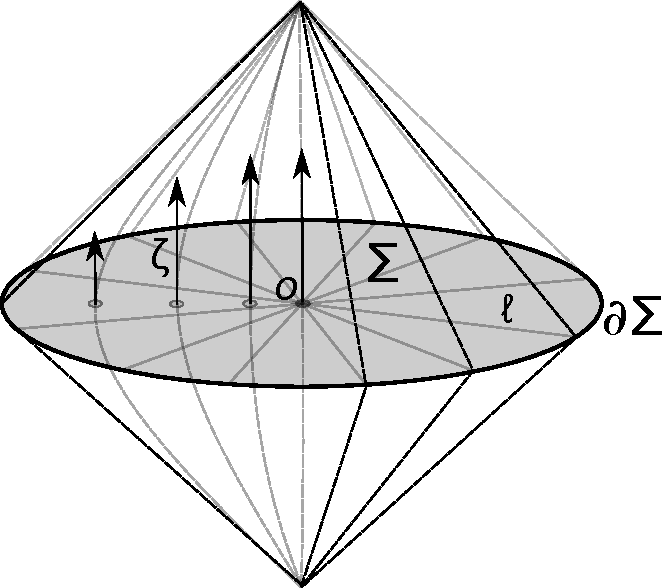
\includegraphics[scale=0.6]{doublecone3.pdf}
%\vspace{-1.5cm}
\caption{Causal diamond, in a maximally symmetric spacetime, for a geodesic ball $\Sigma$ of radius $\ell$ with center $o$ and boundary $\partial \Sigma$. 
The dashed curves are flow lines of $\z$, the conformal Killing vector field, whose flow preserves the diamond
and  which vanishes at the top and bottom vertices and on $\partial\Sigma$.
The vectors show $\z$ at four points of $\Sigma$.}
%\vspace{-3mm}
\label{doublecone}
\end{figure}
%

To connect now with spacetime and the Einstein equation, note that the spatial Ricci scalar 
at $o$ is equal to twice the RNC $00$-component of the spacetime Einstein tensor: 
%
\beq\label{RG00}
{\cal R}=R_{ik}{}^{ik}=R-2R_0{}^0=2(R_{00}-\half R g_{00})=2G_{00}.
\eeq
%
The area deficit \eqref{dAV} can thus also be expressed as 
%
\beq\label{dAVG}
\d A|_V = -\frac{\O_{d-2}\ell^d}{d^2-1} G_{00}.
\eeq
%
%where the Riemann normal coordinate conditions $g_{00}=-1$, $g_{0i}=0$ at $o$ have been used.
%This relation between the sum of the sectional curvatures and the Einstein tensor seems to be Pauli's own observation. 
Then, using the Einstein equation \eqref{Einstein}, 
we see that the area deficit is proportional to the energy density,
%In the Riemann normal coordinate system at $o$, 
%the $00$ component of this equation expresses the proportionality of the spatial Ricci scalar and the 
%energy density $T_{00}$,
%%
%\beq\label{R=T}
%{\cal R} = 16\pi G \,T_{00}.
%\eeq
%%
%This is the well-known scalar initial value constraint equation of general relativity, 
%since by construction the extrinsic curvature of $\Sigma$ vanishes at  at $o$. 
%In terms of the area deficit at constant volume \eqref{dAV}, it takes the form 
%
\beq\label{dAT}
\d A|_V = - \frac{8\pi G\O_{d-2}\ell^d}{d^2-1} \,T_{00}.
\eeq
%
%where the equality holds up to terms of $O(\ell^3)$.
%Pauli's observation, transmitted (or re-discovered) by Feynman\footnote{Feynman expressed it in terms of the radius excess rather than the area deficit.}, 
%is that 
Conversely, this
simple geometrical relation contains the full content of Einstein's equation,
if it holds at all spacetime points and for all timelike unit vectors. 
%then $(G_{ab} - 8\pi G\, T_{ab})u^au^b=0$ for all timelike vectors $u^a$, which in turn implies \eqref{Einstein}.%\footnote{In Section 42-3 of Volume II of the Feynman lectures  \cite{Feynman}, Feynman expressed the Einstein equation in terms of the radius excess of a small sphere: $\d r = GM/3c^2$, where $M$ is the mass contained in the sphere.  rather than the area deficit however. (He did not---and could not, given his audience---mention that the small ball should be generated by spacetime geodesics launched orthogonal to a fixed timelike direction at the center.) I imagine that Feynman may have learned about this it from Section 17 (``Riemannian coordinates and their applications") of Pauli's 1921 review of relativity \cite{PauliEncyc,PauliDover}. Pauli cites Riemann as well as contemporary researchers for the relevant geometrical relations. He is of course quite explicit about the geodesic nature of the ball. While he notes the relation of the spatial scalar curvature at the center of the ball to the Einstein tensor, he does not remark that the Einstein equation can be characterized purely in this manner.}  

The evidence that the Einstein equation implies 
maximal vacuum entanglement can now be stated in a qualitative, intuitive fashion. 
Suppose the ball has a Bekenstein-Hawking entropy $A/4\hbar G$, arising from vacuum entanglement, and we try to increase
the entropy by placing an entangled qbit in the ball. 
To localize the qbit within a region of size $\ell$ we must give it an energy of
at least $\hbar/\ell$ which, according to \eqref{dAT}, will contribute an area deficit of order 
$\hbar G$, hence a surface entropy decrease of order unity, offsetting the
added qbit. It would not help to use a ``highly entropic object" with many internal states, because the existence of such objects makes its mark in
the vacuum as well, diluting the entropic effect of adding the object to the ball. Indeed, in the context of the Rindler wedge, it was argued that $\delta S \le \delta E/T$, where $T$ is the Unruh temperature $\hbar/2\pi$ and $\d E$ is the change of boost Killing energy, since a thermal state maximizes entropy at fixed energy \cite{Marolf:2003sq, Marolf:2004et}.
We now proceed to make this link between the Einstein equation and maximal vacuum entanglement more precise.


\section{Causal diamond and conformal isometry}

To evaluate the variation of the entanglement entropy in a spacelike geodesic ball $\Sigma$ 
it is helpful to consider the spacetime region causally determined by $\Sigma$,
called the {\it causal diamond} $D(\Sigma)$. 
In a maximally symmetric spacetime, $D(\Sigma)$
% is also called the ``double cone":  it 
%is the intersection of the future of $p$ with the past of $q$, where $q$ and $p$ lie at proper times 
%$\pm \ell$ from $o$ along the timelike geodesic through $o$ in the direction $u^a$.  
%In a maximally symmetric spacetime, this diamond 
is the intersection of the future of a past vertex and the past of a future vertex,
and has a conformal isometry and rotational symmetry in the rest frame defined by these vertices
(see Fig.~\ref{doublecone}). 

The Minkowski line element $ds^2 = -dt^2 + dr^2 + r^2d\O^2$ takes the 
form $ds^2 = - du\, dv + r^2d\O^2$ with null coordinates $u=t-r$ and $v=t+r$. 
The Minkowski diamond centered on the origin consists of the intersection of the regions $u>-\ell$ and $v<\ell$. 
The unique conformal isometry that preserves the diamond, and is spherically symmetric, is 
generated by the conformal Killing vector 
%\footnote{Any vector field of the form $\xi=A(u)\partial_u + B(v)\partial_v$ is a conformal isometry of the $du dv$ factor of the metric,  $\L_\xi du dv = [A'(u) + B'(v)]dudv$ (here $\L_\xi$ is the Lie derivative along $\xi$). It is a conformal isometry of the full Minkowski metric if
%$\L_\xi r^2 = [A'(u) + B'(v)] r^2$.  Using $r=(v-u)/2$ we find $\L_\xi r^2 = (B-A)r$, 
%so $\xi$ is a conformal Killing field if $[A'(u) + B'(v)] (v-u)/2 = B(v)-A(u)$. 
%At $u=v$ this implies $B(v)=A(v)$, hence at $v=0$ this condition becomes 
%$[A'(u) + A'(0)] u/2 = A(u)-A(0)$. The general solution is $A(u) = a + bu + cu^2$. 
%The group generated by these vector fields is $SL(2,R)$.
%To map the diamond onto itself, the flow of $\xi$ must leave invariant the boundaries $u=-\ell$ 
%and $v=\ell$. This implies $A(\pm\ell)=0$, hence $A(u) = a(1-u^2/\ell^2)$.}
%
\beq\label{zeta}
\zeta = \frac{1}{2\ell}\bigl[(\ell^2-u^2)\partial_u +(\ell^2-v^2)\partial_v\bigr]
\eeq
% 
(for a derivation see Appendix \ref{AppB}).
Expressed in $t$ and $r$ coordinates, $\zeta$ is given by
%
\beq
\zeta = \frac{1}{2\ell}\bigl[(\ell^2-r^2-t^2)\partial_t -2rt\, \partial_r\bigr].
\eeq
%
The Lie derivative of the Minkowski metric along $\z$ is 
%
\beq\label{Lieg}
\L_\z \eta_{ab} = -(2t/\ell)\, \eta_{ab}.
\eeq
%
The vector $\z$ is tangent to the null generators on the past and future null boundaries of the diamond, 
so those boundaries are  conformal Killing horizons \cite{1979JMP....20..409D}. 
They meet at the ball boundary $\partial\Sigma$, where $\z$ vanishes,
so $\partial\Sigma$ is a bifurcation 
surface.  The surface gravity $\k$ of a conformal 
Killing horizon is well-defined by the equation $\nabla_a \z^2 = -2\k \z_a$ \cite{Jacobson:1993pf}, 
and with the normalization of $\z$ in \eqref{zeta} it is equal to unity. 
%If the Minkowski metric is multiplied by a conformal factor $\psi^2$, $\z$ remains a 
%conformal Killing vector for the diamond, and the surface gravity is unchanged provided
%$\nabla_a \psi^2$ is nonsingular on the horizon.

\section{Entanglement entropy of a diamond}

%We are now ready to consider what happens to the diamond entanglement entropy 

The entanglement entropy in a diamond $D(\Sigma)$ is the same as that in $\Sigma$.
Under a simultaneous variation of the geometry and the state of the quantum fields,
$(\d g_{ab}, \d|\psi\ra)$, the diamond entanglement entropy variation will consist of two 
contributions, a state-independent UV part 
$\d S_{\rm UV}$ from the area change induced by $\d g_{ab}$, and a state-dependent 
IR part $\d S_{\rm IR}$ from $\d|\psi\ra$. 

As mentioned above, we are assuming that, as a result of the UV physics, the entanglement entropy in a spatial
region is finite in any state, with a leading term $\eta A$. Here $A$ is the area of the boundary of the region and 
$\eta$ is a universal constant with dimensions [length]${}^{2-d}$.
%, the surface entanglement density of the vacuum. 
The scaling with area is natural in any theory with a large density of states at short distances. The assumption that $\eta$ is universal is motivated by the idea that the UV structure of the vacuum is common to all states in the class being considered.\footnote{This involves an implicit choice of ``conformal frame" \cite{Flanagan:2004bz} for the metric, namely, the one for which $\eta$ is constant in spacetime. This metric turns out to satisfy the Einstein equation, so this frame is the so-called ``Einstein frame".}
%\footnote{In the presence of non-minimal coupling terms such as $\vphi^2 R$ or a dilaton coupling $e^{-2\phi} R$ in the Lagrangian, the entropy would depend on the vacuum expectation value of $\vphi^2$ or $e^{-2\phi}$, which could vary over spacetime. In this case, either $\eta$ and the effective local value of the gravitational constant would vary, or one could make a compensating Weyl rescaling of the definition of the metric field.} 
%There will also be sub-leading, state-dependent \cite{Cooperman:2013iqr} contributions to the entropy. These would presumably be suppressed by the ratio $(\l_{\rm UV}/\l_{\rm curvature})^2$.
%We thus assume that, when 
Under this assumption, when the geometry is varied, the contribution to the entanglement entropy in 
$\S$ from the UV degrees of freedom near the boundary  $\partial\Sigma$
changes by an amount
%
\beq\label{SUV}
\d S_{\rm UV}=\eta\, \d A. 
\eeq
%
The total entropy variation will thus be given by 
%
\beq\label{dStot1}
\d S_{\rm tot} = \eta\, \d A + \d S_{\rm IR}
\eeq
%
If $\eta=1/4\hbar G$, \eqref{SUV} coincides with 
the variation of Bekenstein's generalized entropy, here interpreted as simply the total entropy in the diamond.
The MVEH implies that the total entropy variation \eqref{dStot1} is zero at first order , and negative for finite 
variations, when comparing to a maximally symmetric spacetime with 
the volume of $\S$ held fixed. 

To motivate this equilibrium condition,
we first recall that, 
%The need to fix the volume is familiar from ordinary thermodynamic systems. 
%, which in equilibrium minimizes a free energy function. 
%For example, 
for ordinary thermodynamic systems
in equilibrium, the Helmholtz free energy $F=E - TS$ is minimized at fixed volume.
The MVEH is analogous, but with the additional feature that the energy 
vanishes.
%(and fixed charges that might contribute to chemical potential terms). 
%If $E$ is fixed, the entropy increases with volume, hence the necessity of fixing the volume.
%The entropy can also be increased by increasing $E$ at fixed volume but, thanks to the $E$-term, 
%$F$ will nevertheless increase. 
%If $E$ and the volume are both fixed, then the entropy must be maximal, otherwise $F$ could be decreased. 
That the free energy of a diamond has no energy term can be motivated by 
comparison with de Sitter spacetime, and the restriction to fixed volume arises from 
the fact that the diamond has a conformal Killing vector rather than a true Killing vector (see Appendices \ref{AppC} and \ref{AppD}). 


%A small diamond %is surrounded by a conformal Killing horizon. In fact it 
%is conformally isometric to a static patch of dS. %, which is 
%%bounded by the dS Killing horizon. %I propose that this similarity with dS provides the way to understand its free energy.  
%The quantum statistical mechanics of dS was considered long ago by 
%Gibbons and Hawking \cite{Gibbons:1976ue}. They examined the thermal partition function and argued that, since Euclidean dS is closed, the mass, angular momentum, and electric charge vanish, so that the only term in the free energy for pure dS space is the entropy term, $F_{\rm dS}=-TS$. The minimization of dS free energy is thus equivalent to the maximization of entropy. % in this case, and that is what I will assume for small causal diamonds.
%This result can also be understood via the ``first law of event horizons" \cite{Gibbons:1977mu}.
%For a Schwarzschild black hole, this law would read $\d M = (\k/8\pi G)\d A + \d E_K$, where  $M$ is the mass, $\k$ and $A$ are the surface gravity and horizon area of the black hole, and $E_K$ is the Killing energy of a matter fluid 
%surrounding the black hole \cite{Bardeen:1973gs}. 
%For dS, instead the first law reads
%%
%\beq\label{dS1st}
%(\k/8\pi G)\d A + \d E_K=0.
%\eeq
%% 
%There is no geometric total energy term since there is no asymptotic region. 
%The vanishing of the 
%total entanglement entropy variation \eqref{dStot1} is directly analogous to the first law of horizon mechanics 
%in de Sitter space \eqref{dS1st}. In fact, one can derive a classical first law of flat causal diamonds, which has the form \eqref{dS1st} with $\d A$ replaced by $\d A|_V$ \eqref{dAV}. The $\d V$ term arises from the fact that the diamond 
%has a conformal Killing vector rather than a true Killing vector \cite{DiamondSupplement}.

%In General Relativity, because of diffeomorphism invariance, the total energy, i.e.\ the value of the Hamiltonian generating time evolution, is just a boundary term. 
%In dS the only boundary for the static patch is the horizon, and the contribution from the horizon is equal to 
%$-TdS$, where $T$ and $S$ are the dS temperature and entropy. 



%The first law \eqref{dS1st} is very close to what we will impose for the diamond, once we relate the IR entropy variation to the conformal Killing energy variation. There is, however, an important difference: we must fix the volume. This difference originates in the fact that the diamond has only a {\it conformal} Killing vector \eqref{Lieg}, not a true Killing vector. Because of this, the first law of the diamond contains an extra term not present in \eqref{dS1st}. The technical origin of this extra term will be explained at the end of this paper, but its necessity can be immediately seen as follows. If there is no matter, \eqref{dS1st} implies that in any variation of dS space, $\d A = 0$, whereas 
%the same is obviously not true for a small diamond in Minkowski spacetime. (Here I am invoking a strong form of \eqref{dS1st} that applies to all variations \cite{Iyer:1994ys}, not only to variations to another stationary solution.)  The need to hold the volume fixed is analogous to that for an ordinary thermodynamic system. 

%\section{Entanglement entropy of small diamonds}

Our next step is to evaluate $\d S_{\rm IR}$.
The vacuum state of any QFT, restricted to the diamond, can be expressed (formally) as a
thermal density matrix, 
%
\beq\label{rK}
\r = Z^{-1}\exp(-K/T),\quad T=\hbar/2\pi,
\eeq
%
where $K$ is the ``modular Hamiltonian".  
The temperature $T=\hbar/2\pi$ is factored out here so that $K$ will be the 
generator of Lorentz boosts, i.e.\ hyperbolic angle shifts, at the edge of the diamond. 
For an infinite diamond that coincides with the Rindler wedge in Minkowski space, 
$T$ is the Unruh temperature \cite{Unruh1976, Sewell1982}.

%(It has dimensions of action because the Hamiltonian generates the flow of a dimensionless parameter---hyperbolic angle in the case of the wedge.) 


Because $\r$ in \eqref{rK} has the form of a thermal state, it minimizes the modular free energy, 
%
\beq\label{FK}
F_K =\la K\ra - TS,
\eeq
%
where  the brackets denote quantum expectation value, and $S=-\Tr \r\ln\r$ is the von Neumann entropy. 
The variation $\d F_K$ must therefore vanish for any small variation  $\d\r$ of the state, i.e.\  
%
\beq\label{dSK}
\d S = \frac{2\pi}{\hbar}\d \la K\ra.
\eeq
%
This is just the usual Clausius relation for a ``thermal" state \eqref{rK}.

In general  $K$ in \eqref{rK} is not a local operator, and does not generate a geometric flow.
For a CFT, however, $K$ is equal to $H_\z$, the Hamiltonian generating the 
flow of the conformal boost Killing vector \eqref{zeta} \cite{Hislop:1981uh}. 
%(This has provided the method for evaluating the entanglement entropy in 
%a spherical ball in the CFT dual to the bulk gravity theory in the AdS/CFT setting \cite{Casini:2010kt}.)
(This result is conformally related to the better-known version that holds for any
Poincar\'e invariant QFT restricted to the Rindler wedge \cite{Bisognano:1976za}.)
%which holds for any Poincare invariant field theory. In the wedge, the Hamiltonian generating 
%the flow is the Lorentz boost generator. The temperature $T=\hbar/2\pi$ is the universal vacuum temperature of a horizon.
%(It has dimensions of action because the Hamiltonian generates the flow of a dimensionless parameter---hyperbolic angle in the case of the wedge.) 
%The conformal boost generator can be expressed as an integral of the conformal boost energy current 
%$J_\z^a=T^{ab}\z_b$, 
That is, $H_\z$ is given by the integral
%
\beq\label{Hz}
H_\z = \int_\Sigma T^{ab} \z_b\, d\Sigma_a.
\eeq
%
%The divergence of the current $J_\z^a$ is $\nabla_a J_\z^a = (\nabla_a\z^a)\frac{1}{d} T$, where $T=T^{ab}g_{ab}$ is the trace. For a CFT, the trace is a state-independent constant (or vanishes if there is no anomaly), so up to a c-number the integral in \eqref{Hz} gives the same result when evaluated on any surface whose boundary is $\partial\S$.
%
%We  now exploit this geometrical interpretation of $K$ to evaluate $\d\la K\ra$.
%It is commonly evaluated on the $t=0$ surface, but it can
%also be evaluated on the lower null cone $\cal C^-$ bounding the diamond. 
If the quantum field state is varied away from the vacuum, with an excitation length scale much 
longer than the diamond size, 
%
\beq\label{lexcitation}
\ell \ll L_{\rm excitation},
\eeq
%%
then $\la T_{ab}\ra$ can be treated as constant, and 
using the Killing field \eqref{zeta}
we find
%
\beq\label{dHz}
\d \la H_\z\ra =\frac{\O_{d-2} \ell^d }{d^2-1}\, \d\la T_{00}\ra.
\eeq
%

If the matter field is {\it not} conformal, $K$ is not given by \eqref{Hz}, and we cannot directly use \eqref{dHz}.
%Even in a diamond much smaller than any length scale in the QFT, so that the effect of masses might be negligible,
%the interaction coupling constants run logarithmically with scale, which likely precludes the use of conformal symmetry 
%in the diamond interior. 
However, suppose that the matter is described by a QFT with a UV fixed point, so it is 
asymptotically conformal at short distances, and that, in addition to \eqref{lexcitation}, 
the diamond is much smaller than 
any length scale in the QFT, 
%
\beq
\ell\ll L_{\rm QFT}.
\eeq
%
Then we conjecture---and we shall assume---that $\d \la K\ra$ 
%is the same as \eqref{dHz}, except with $T_{ab}$ replaced by its tracefree part, 
has the form of  \eqref{dHz} with an additional term $\d X$ that is a spacetime scalar,
%proportional to the variation of the expectation value of a scalar operator,
%
\beq\label{dKC2}
\d \la K\ra =\frac{\O_{d-2} \ell^d }{d^2-1}\, \bigl(\d\la T_{00}\ra+\d X\bigr).
\eeq
%
(The common coefficient is factored out to simplify later expressions.)
Calculations \cite{Casini:2016rwj,Speranza:2016jwt} indicate that for a class of theories and states,
this is the case, although in general 
$\d X$ may carry $\ell$ dependence and can dominate at small $\ell$.\footnote{In 
a previous draft of this paper, I had conjectured that $X=-\frac1d \la T\ra$, 
so that what appeared in $\d\la K\ra$ would be just the tracefree part of $\la T_{ab}\ra$.} 
Note that the relation \eqref{dKC2} refers only to the expectation value, and only to 
lowest order in the radius of the ball.

%Calculations by Damian Galante \cite{Damian} and Antony Speranza \cite{Antony} 
%Calculations \cite{Damian,Antony} 
%indicate that is not the case. However, it suffices for the derivation that $X$ be any scalar operator.


%(A CFT trace anomaly $\la T\ra$ is independent of the state, so that $\d\la T\ra$ = 0 in that case.)

%Another way to state this is that we should carry out the integral in \eqref{Hz} not over $\Sigma$ but over 
%the lower (or upper) null cone $\cal C$ bounding the diamond, since then only the null-null component
%$T_{vv}$ (which depends only on the tracefree part) enters. Stated this way, the conjecture can 
%at most be valid on diamonds small enough for $T$ to be treated as constant. To see why, 
%note that the upper and lower cones are on equal footing in computing $\d\la K\ra$,  so the integrals 
%of $\d\la J_z^a\ra$ over the two cones had better be equal, where $J_\z^a=T^{ab}\z_b$
%is the boost energy current.  The difference of these two surface integrals is the spacetime
%volume integral of the divergence $\nabla_a \d \la J_\z^a\ra=\frac{1}{d}\d\la T\ra\nabla_a\z^a$.  
%For a CFT the trace $T$ can arise only from a state-independent anomaly, so its state-variation 
%$\d\la T\ra$ vanishes. For a general QFT, the difference of the surface integrals vanishes
%if $\d\la T\ra$ is constant, since then it is proportional to the integral of $\nabla_a\z^a$,
%and the null vector $\z^a$ has vanishing contraction with the null 
%integration measure $d\Sigma_a$ on the cones.

%Some support for this entanglement variation conjecture exists. For one thing, 
%when restricted to the null planes bounding the Rindler wedge in Minkowski spacetime,  
%the algebra and vacuum state of a free massive scalar or spinor field is independent of the 
%mass of the field (see, e.g.\ \cite{Wall:2011hj}).
%Further evidence comes from a result \cite{Fredenhagen:1984dc}
%relating the modular flow of the vacuum in a diamond to the boost flow of a Rindler wedge to which it is tangent on both cones. For any asymptotically scale invariant QFT,  the two flows coincide in the limit that the initial operator algebra is restricted to successively smaller and smaller neighborhoods of the corner of the wedge.
%On the other hand, we cannot take the diamond so small that it approaches the Planck length where presumably 
%no well defined classical background geometry exists. Hence we should expect corrections to \eqref{dKC2}. 
%The largest corrections would be not
%from a mass scale in the QFT, but from a logarithmic approach to scale invariance, as in QCD.
%If this were to produce a correction of order $\sim 1/\ln(L_{\rm QFT}/\ell)$, that would be nonnegligible.
%We leave it to future work to either verify or invalidate Eq.~\eqref{dKC2} for, say, the fields of the standard model.
 
%in the case of constant $\la T_{ab}\ra$. 
%If it is false, the derivation of this paper fails. 

%On $\cal C$,  $u=-\ell$, so the Killing field \eqref{zeta} 
%is the null vector $\frac{1}{2}(1-v^2)\partial_v$, in units with $\ell=1$. The light cone integration measure is
%$d\Sigma^a = \partial_v^a r^{d-2} dv d\O$. The integral \eqref{dKC} thus involves only the null-null $T_{vv}$ component, 
%so depends only on the tracefree part of the energy-momentum tensor, $T_{ab}-\frac{1}{d}Tg_{ab}$. 
%Carrying out the integral, we find 
%%
%\beq\label{dKC2}
%\d \la K\ra =\frac{\O_{d-2} \ell^d }{d^2-1}\, (\d\la T_{00}\ra-\frac{1}{d}\d\la T\ra g_{00}).
%\eeq
%%
%If $\la T_{ab}\ra=0$ in the equilibrium state, then we can omit the variation symbol $\d$; however, for conceptual clarity and generality we maintain the $\d$. %With this result in hand we can now put the pieces together.


%\section{Maximal entropy and the Einstein equation}
\section{Equilibrium and the Einstein equation}

We now postulate that a small diamond is in equilibrium if the quantum fields are in their vacuum state, and the curvature is that of a maximally symmetric spacetime (MSS) (Minkowski or (anti)-de Sitter). 
Any MSS seems an equally good candidate, so we will regard the curvature scale of the MSS as a local state parameter that is effectively constant in a small diamond but may 
depend on the diamond. 
%vary in spacetime. 

The Einstein tensor in a MSS is $G^{\rm MSS}_{ab}=-\l g_{ab}$, with $\l$ a curvature scale. When the metric is varied away from the MSS, the area variation at fixed volume is obtained to lowest order in curvature by replacing $G_{00}$ in \eqref{dAV} with $G_{00}-G^{\rm MSS}_{00}$, which yields 
%
\beq\label{dAVGrel}
\d A|_{V,\l} = -\frac{\O_{d-2}\ell^d}{d^2-1} (G_{00}+\l g_{00}).
\eeq
%
The variation of the total diamond entropy \eqref{dStot1} 
away from the equilibrium can now be written using
\eqref{dAVGrel}, \eqref{dSK} , and \eqref{dKC2}:
%
\begin{align}
\label{dStot2}
\d S&_{\rm tot}|_{V,\l}=\eta\, \d A|_{V,\l}+\frac{2\pi}{\hbar}\d\la K\ra
= \frac{\O_{d-2}\ell^d}{d^2-1}\times\nonumber\\ 
&\left[-\eta \,(G_{00} +\l g_{00})+\frac{2\pi}{\hbar}\bigl(\d\la T_{00}\ra+\d X\bigr)\right].
\end{align}
%
The Einstein tensor should presumably be understood here as a quantum expectation value $\la G_{ab}\ra$, since the entropy that is maximized is, by definition, an expectation value.
In using \eqref{dKC2} for the matter entanglement variation, we are neglecting corrections that
would come from the curvature of the MSS, since those would be of higher order.

The requirement that the variation \eqref{dStot2} vanishes at all points and with all timelike unit vectors implies a tensor equation,
%
\beq\label{attempt1}
G_{ab} +\l\,g_{ab}= \frac{2\pi}{\hbar\eta}\bigl(\d\la T_{ab}\ra+\d X g_{ab}\bigr).
\eeq
%
The divergence of this equation, together with the Bianchi identity and local conservation of energy,  ties 
$\l$ to $\d X$ via
%
\beq\label{tie}
\l = \frac{2\pi}{\hbar\eta}\d X + \Lambda,
\eeq
%
where $\Lambda$ is a spacetime constant. 
Had we not allowed for the MSS curvature scale $\l$ in the equilibrium state,
\eqref{tie} would have implied the unphysical restriction that the scalar term $\d X$ be constant. Note also that
if $\d X$ has $\ell$-dependence then so does $\l$.

When \eqref{tie} is substituted back into \eqref{attempt1} we arrive at
%
\beq\label{bingo}
G_{ab} +\Lambda \,g_{ab}= \frac{2\pi}{\hbar\eta}\d\la T_{ab}\ra.
\eeq
% 
This is Einstein's equation with an undetermined cosmological constant $\Lambda$, which evidently must 
be independent of $\ell$,
and with Newton's constant defined by 
%
\beq
G=\frac{1}{4\hbar\eta}.
\eeq
%
The area density of entanglement entropy $\eta$ and Planck's constant thus determine the gravitational coupling strength.
Stronger vacuum entanglement implies weaker gravity, i.e.\ greater spacetime rigidity. 
Note the crucial consistency: When expressed using $G$, the surface entropy $\eta A$ is the Bekenstein-Hawking entropy 
$A/4\hbar G$. The coefficient would have been off by the factor $(d+1)/3$ had we used the area variation at fixed
radius \eqref{dA} rather than at fixed volume \eqref{dAV}. 



%\section{First law of causal diamond mechanics}
%The total entanglement entropy variation \eqref{dStot2} is directly analogous to the first law of horizon mechanics 
%in de Sitter space \eqref{dS1st}.
%This suggests that there should be a strictly classical limit of our result. In fact, there is indeed a first law of causal diamond mechanics, and it further illuminates why we must consider variations at fixed volume.
%%, and it is helpful in understanding why we must hold the volume fixed in our derivation. 
%%Previously laws of horizon mechanics have been derived for variations away from solutions with a bifurcate Killing horizon, but we can generalize this to encompass conformal Killing horizons as follows. The Noether current $j_\xi$ associated with any vector field $\xi$ is exact on shell for any diffeomorphism invariant gravity theory, and it follows that $j_\xi = dQ_\xi$ for some Noether charge ($d-2$)-form built locally from the fields and their derivatives \cite{Wald}.
%%Now c
%
%Consider a causal diamond in any conformally flat solution to Einstein's equation (this can be generalized to any diffeomorphism invariant gravity theory). There is a conformal Killing vector $\z$ that preserves the diamond, and for which the edge of the diamond is the bifurcation surface. Hence we may invoke the variational identity 
%%
%\beq\label{1stlaw}
%\d H_\z = \d \oint_{\partial\Sigma} dQ_\z,
%\eeq
%%
%where $H_\z$ is the conformal boost Hamiltonian generating evolution along the flow of $\z$ (constructed from the symplectic 
%form evaluated on the Lie derivative of the fields along $\z$), and the variation is to any neighboring solution \cite{Iyer:1994ys}. The surface integral yields $-\k \d A/8\pi G$ as usual. If $\z$ were a Killing vector, $\d H_\z$ would vanish for all fields invariant under the Killing flow.
%%, because it is linear in the Lie derivative of the background solution with respect to $\z$. 
%For matter treated as a fluid, it would not vanish, because the fluid potentials do not share the symmetry of the metric \cite{Iyer:1996ky,Green:2013ica}. Thus, for example, if the diamond were the static patch of de Sitter space, we would recover in this way the first law of de Sitter horizons \eqref{dS1st}.
%
%Since $\z$ is only a conformal Killing vector,  $\d H_\z$ receives contributions both from matter and from the gravitational field. If the background solution is Minkowski spacetime, the gravitational field contribution is 
%$-(d-2)\k\d V/8\pi G\ell$.
%(The expression for the symplectic form in \cite{Hollands:2012sf} is helpful for computing this.) When combined with the area variation term, this yields the area variation $\d A|_V$ at fixed volume \eqref{dAV}. 
%Moreover, the conformal boost energy of the matter integrated over $\Sigma$ is given by the right hand side of \eqref{dAT}, when $T_{00}$ is constant. In this way we see that \eqref{1stlaw} recovers the statement of \eqref{dAT}, that addition of matter energy to the diamond decreases the area of the boundary at fixed volume.

\section{Discussion}

We have shown, given our assumptions, that the semiclassical Einstein equation 
holds, 
for first-order  variations of the vacuum, 
if and only if the entropy in small causal diamonds is stationary at constant volume, when varied from a maximally symmetric vacuum state of geometry and quantum fields. 
We assumed the diamond size $\ell$ is much smaller than the local curvature length, 
the wavelength of any excitations of the vacuum, and
the scales in the matter field theory, but much larger than the UV scale at which quantum gravity effects become strong.
Our entanglement variation assumption for nonconformal matter \eqref{dKC2} 
%(with constant $\la T_{ab}\ra$) 
concerns only standard QFT, and is either true or false. 
%If it is false, the argument collapses, though could perhaps be reconstructed on a different support. 

Strictly speaking the ``first-order  variation" refers to the derivative with respect to a parameter labeling the state, evaluated at the vacuum. To be physically applicable, however, the result should apply to finite but small variations. The example of a coherent state reveals a challenge in this regard \cite{Madhavan}: Such a state can have nonzero energy density while leaving entanglement entropy unchanged \cite{Fiola:1994ir, Benedict:1995yp}. That is, not all energy registers as a change of entanglement. This is consistent with the hypothesis of maximal vacuum entanglement, although the Einstein equation implies that the entropy has decreased --- relative to vacuum --- by more than it needs to in order to satisfy the hypothesis. Unless a further consequence of that hypothesis is found, or the hypothesis is refined and strengthened in some way, the Einstein equation does not appear to follow from it in all generality.

We close with some questions and remarks concerning the derivation and its implications.

\begin{itemize}

\item Do graviton fluctuations contribute to the entanglement entropy? 
The UV part of the entanglement entropy $S=\eta A$ is inscrutable  at this level,
%It might include graviton entanglement. 
and the IR part does not include gravitons. Since the diamond is taken much smaller than the wavelength of any ambient gravitons, 
they have no gauge-invariant meaning in the diamond. In the RNC gauge they are absent at first derivative order.
%no meaningful stress-energy tensor could be attributed to the gravitons. 
Moreover, the full, nonlinear Einstein tensor already appears on the geometric side of the equation, 
so it would be double counting to include any graviton energy. 

\item Can a gravitational field equation with higher curvature corrections be derived along these lines? Maybe.  
We neglected terms of order $\ell/L_{\rm curv}$ in the geometry calculations, whereas a next-higher-curvature correction to the field equation might be of order $(\ell_1/L_{\rm curv})^2$, where $\ell_1^2$ is the relative coefficient of the curvature squared term in the action. To capture this within our approximation would require $\ell/\ell_1<\ell_1/L_{\rm curv}$. The right-hand side is presumably less than unity, in order for higher-curvature terms to not dominate, so the diamond would have to be taken smaller than $\ell_1$.  If, say, $\ell_1$ were the string length,
would classical geometry and quantum field theory apply at that scale? Probably not. On the other hand, perhaps with improved accuracy of the geometric analysis, and the inclusion of subleading UV terms in the entanglement entropy, one could consistently capture higher-curvature corrections using a diamond larger than $\ell_1$.

%\item Our stationary entropy assumption ({\it iii}) follows from the stronger assumption that the diamond entropy $S_{\rm tot}$ is locally {\it maximal} in the maximally symmetric vacuum state at fixed volume. Does the Einstein equation imply this stronger condition? This question can be posed both classically and semiclassically.
%%To investigate this one could examine the second variation of the diamond entropy, both classically \cite{Hollands:2012sf}.  

\item A derivation of Einstein's equation invoking a quantum limit to measurements of the spacetime geometry of small causal diamonds was given in Ref.~\cite{Lloyd:2012du}. How are the assumptions used there related to those made here?

%\item If the Einstein equation expresses entropy maximization, what then is the role of energy? Energy enters our derivation through the diamond modular Hamiltonian $K$, which is just (minus) the logarithm of the matter field density matrix. This suggests the that  energy density derives from entanglement entropy. A corollary would be that time, which is conjugate to energy, derives from the modular flow. This would be a local realization of the thermal time hypothesis \cite{Rovelli:1993ys,Connes:1994hv} in each diamond \cite{Martinetti:2002sz}.

\item According to our derivation the Einstein equation is a property of vacuum equilibrium. 
Does this suggest how to include nonequilibrium effects? 

\end{itemize}

\vspace{3mm}
\acknowledgments

I am very grateful to H. Casini, W.~Donnelly, C.T.~ Eling, S.~Hollands, J.~Maldacena, D.~Marolf, M.~van Raamsdonk, V. Rosenhaus, C.~Rovelli, A. Satz, A.~Speranza, J. Suh, M. Varadarajan, and A.~Wall for helpful discussions, comments, and suggestions, and to anonymous referees for comments that led me to improve the presentation. This research was supported in part by the National Science Foundation under Grants No.\ PHY-1407744, and No.\ PHY11-25915.

\appendix

\section{Area deficit calculation}
\label{AppA}

%In this section we provide 
%some details in the derivation of the area deficit that were omitted in the main text,
%and add some comments and references. 

For the Riemann normal coordinate (RNC) system based at a point $o$
we let $x^0$ denote the timelike coordinate and let $\{x^i=r n^i\}$ denote the 
spacelike coordinates, where $r$ is the geodesic distance and $n^i$ is a unit vector at $o$, 
$\d_{ij}n^i n^j=1$. The components of the metric at $o$ in this coordinate system are
$g_{00}=-1$, $g_{0i}=0$, and $g_{ij}=\d_{ij}$.  The spacelike geodesic ball of radius 
$\ell$ is denoted $\Sigma$. 
By definition, $\Sigma$ lies within the $x^0=0$ surface in this coordinate system. 
Using the standard result for the RNC metric components, 
the spatial metric $h_{ij}$ on $\Sigma$ takes the form 
%
\beq\label{metric}
h_{ij} = \d_{ij} -\tfrac{1}{3} r^2 R_{ikjl}\,n^k n^l + O(r^3)
\eeq
%
where $R_{ikjl}$ are the spatial components of the spacetime Riemann tensor evaluated at $o$.
The extrinsic curvature of $\Sigma$ vanishes at $o$, 
since $\Sigma$ is generated by geodesics from $o$. The components $R_{ikjl}$ are therefore 
also equal to the components of the spatial Riemann tensor. 

To lowest nontrivial order in the ratio $\ell/L_{\rm curvature}$
the volume element of $\Sigma$  is 
%
\beq\label{sqrth}
dV =\sqrt{h}\, d^{d-1}x =(1 - \tfrac16 r^2 R_{ik}{}^{i}{}_l\, n^k n^l)r^{d-2}dr\, d\O,
\eeq
%
where $d\O$ is the area element on the unit $(d-2)$-sphere.  
The integral over $d\O$ yields
%
\beq\label{intnn}
\int d\O \,n^kn^l = \frac{\O_{d-2}}{d-1}\d^{kl},
\eeq
where 
$\O_{d-2}$ is the area of the unit $(d-2)$-sphere. For spherically
symmetric integrands, the volume element is therefore 
%
\beq\label{sqrthr}
dV =\O_{d-2}\left(1 - \frac{r^2{\cal R}}{6(d-1)}\right)r^{d-2}dr,
\eeq
%
where ${\cal R}=R_{ik}{}^{ik}$ is the spatial Ricci scalar  at $o$.
Integrating \eqref{sqrthr} over $r$ from 0 to $\ell$ yields 
the volume variation at fixed radius written in the main text, 
%
\beq\label{dV}
\d V|_{\ell} = -\frac{\O_{d-2}\ell^{d+1}}{6(d-1)(d+1)}{\cal R},
\eeq
%
where ${\cal R}=R_{ik}{}^{ik}$ is the spatial Ricci scalar  at $o$.

In the main text, the relation \eqref{dV} is used to find the area variation
at fixed radius and at fixed volume, and the link to the Einstein
equation is made using the relation ${\cal R}=2G_{00}$, where 
$G_{ab}$ is the Einstein tensor.
The viewpoint here is not new. One can find 
the area and volume deficits at fixed radius, and the relation to the Einstein tensor,  
in Section 17 (``Riemannian coordinates and their applications") of Pauli's 1921 review of relativity \cite{PauliEncyc}.
 Pauli cites Riemann, as well as contemporary researchers, for the relevant geometrical relations.  He does not remark that the Einstein equation can be characterized purely in this manner. 
Feynman (in Section 11.2 of \cite{FeynmanGrav} and Section 42-3 of \cite{Feynman}) 
 expressed the Einstein equation for $d=4$ as the statement that, for all timelike directions,
the radius excess (equivalently the radius variation at fixed area) of a small sphere is given by  
$\ell - \sqrt{A/4\pi}=\d \ell|_A = GM/3c^2$, where $M=T_{00}V$ is the ``mass" contained in the sphere.
This can be derived from the relations above using %\eqref{dA} 
[Eq. (4), main text]
together with 
$\d A|_\ell/A = -(d-2)\d \ell|_A/\ell$. 


%At any spacetime point $o$ choose an arbitrary timelike unit vector $u^a$, and generate a $(d-1)$-dimensional spacelike ball $\Sigma$ by sending out geodesics of length $\ell$ from $o$ in all directions orthogonal to $u^a$. 
%The point $o$ is the center of the ball, and the boundary $\partial \Sigma$ is the surface. 
%Choose a Riemann normal coordinate (RNC) system based at $o$, launched from an orthonormal basis formed by 
%$u^a$ and $d-1$ spacelike vectors tangent to $\Sigma$.  Let the timelike coordinate be $x^0$, and
%let the spacelike ones be $\{x^i=r n^i\}$, where $r$ is the geodesic distance and $n^i$ is a unit vector at $o$, 
%$\d_{ij}n^i n^j=1$. The components of the metric at $o$ in this coordinate system are
%$g_{00}=-1$, $g_{0i}=0$, and $g_{ij}=\d_{ij}$. The signature of the spacetime metric is taken here to be $({-}{+}{+}{+})$, and units are chosen with $c=1$.
%
%By definition, $\Sigma$ lies within the $x^0=0$ surface in this coordinate system. 
%Using the standard result for the RNC metric components, 
%the spatial metric $h_{ij}$ on $\Sigma$ takes the form 
%%
%\beq\label{metric}
%h_{ij} = \d_{ij} -\tfrac{1}{3} r^2 R_{ikjl}\,n^k n^l + O(r^3)
%\eeq
%%
%where $R_{ikjl}$ are the spatial components of the spacetime Riemann tensor evaluated at $o$.
%The extrinsic curvature of $\Sigma$ vanishes at $o$, 
%since $\Sigma$ is generated by geodesics from $o$. The components $R_{ikjl}$ are therefore 
%also equal to the components of the spatial Riemann tensor. 
%
%We will assume the radius ball is much smaller than the local curvature length,
%%
%\beq
%\ell\ll \lambda_{\rm curvature}
%\eeq
%% 
%and work to lowest nontrivial order in their ratio. 
%The volume element of $\Sigma$  is thus
%%
%\beq\label{sqrth}
%dV =\sqrt{h}\, d^{d-1}x =(1 - \tfrac16 r^2 R_{ik}{}^{i}{}_l\, n^k n^l)r^{d-2}dr\, d\O,
%\eeq
%%
%where $d\O$ is the area element on the unit $(d-2)$-sphere.  
%The integral over $d\O$ yields
%%
%\beq\label{intnn}
%\int d\O \,n^kn^l = \frac{\O_{d-2}}{d-1}\d^{kl},
%\eeq
%where 
%$\O_{d-2}$ is the area of the unit $(d-2)$-sphere. For spherically
%symmetric integrands, the volume element is therefore 
%%
%\beq\label{sqrthr}
%dV =\O_{d-2}\left(1 - \frac{r^2{\cal R}}{6(d-1)}\right)r^{d-2}dr,
%\eeq
%%
%where ${\cal R}=R_{ik}{}^{ik}$ is the spatial Ricci scalar  at $o$.
%The volume variation at fixed radius is thus given by
%%
%\beq\label{dV}
%\d V|_{\ell} = -\frac{\O_{d-2}\ell^{d+1}}{6(d-1)(d+1)}{\cal R},
%\eeq
%%
%where ${\cal R}=R_{ik}{}^{ik}$ is the spatial Ricci scalar  at $o$.
%The area variation of $\partial\Sigma$ is given by $d\d V/d\ell$, i.e.\ 
%%
%\beq\label{dA}
%\d A|_{\ell} = -\frac{\O_{d-2} \ell^d }{6(d-1)}{\cal R}.
%\eeq
%%
%
%To vary the metric with the volume but not the area held fixed, the radius 
%of the ball must be varied. Then, in addition to the previous contributions arising from the curvature, 
%the volume and area variations have the contributions
%$\d_r V = \ell^{d-2}\int \d r\, d\O$ and $\d_r A = (d-2)\ell^{d-3}\int \d r\, d\O$.
%Choosing $\int \d r\, d\O$ so that the total volume variation vanishes, 
%we obtain the area variation at fixed volume,
%%
%\beq\label{dAV}
%\d A|_V = \d A - \frac{d-2}{\ell}\d V=
%-\frac{\O_{d-2}\ell^d}{2(d^2-1)} {\cal R}. 
%\eeq
%%
%This is smaller in magnitude than the variation at fixed radius \eqref{dA} by the factor 
%$3/(d+1)$.
%
%To connect now with spacetime and the Einstein equation, note that the spatial Ricci scalar 
%at $o$ is equal to twice the RNC $00$-component of the spacetime Einstein tensor: 
%%
%\beq\label{RG00}
%{\cal R}=R_{ik}{}^{ik}=R-2R_0{}^0=2(R_{00}-\half R g_{00})=2G_{00}.
%\eeq
%%
%The area deficit \eqref{dAV} can thus also be expressed as 
%%
%\beq\label{dAVG}
%\d A|_V = -\frac{\O_{d-2}\ell^d}{d^2-1} G_{00}.
%\eeq
%%
%%where the Riemann normal coordinate conditions $g_{00}=-1$, $g_{0i}=0$ at $o$ have been used.
%%This relation between the sum of the sectional curvatures and the Einstein tensor seems to be Pauli's own observation. 
%Then, using the Einstein equation, 
%%
%\beq\label{Einstein}
%G_{ab} = 8\pi G\, T_{ab},
%\eeq
%%
%we see that the area deficit is proportional to the energy density,
%%In the Riemann normal coordinate system at $o$, 
%%the $00$ component of this equation expresses the proportionality of the spatial Ricci scalar and the 
%%energy density $T_{00}$,
%%%
%%\beq\label{R=T}
%%{\cal R} = 16\pi G \,T_{00}.
%%\eeq
%%%
%%This is the well-known scalar initial value constraint equation of general relativity, 
%%since by construction the extrinsic curvature of $\Sigma$ vanishes at  at $o$. 
%%In terms of the area deficit at constant volume \eqref{dAV}, it takes the form 
%%
%\beq\label{dAT}
%\d A|_V = - \frac{8\pi G\O_{d-2}\ell^d}{d^2-1} \,T_{00}.
%\eeq
%%
%Conversely, this
%simple geometrical relation contains the full content of Einstein's equation,
%if it holds at all spacetime points and for all timelike unit vectors. 
%
%The viewpoint here is not new. One can find many of these relations in 
%Section 17 (``Riemannian coordinates and their applications") of Pauli's 1921 review of relativity \cite{PauliEncyc}. Pauli cites Riemann as well as contemporary researchers for the relevant geometrical relations.  
%He describes the scalar curvature as the sum of the sectional curvatures, and notes the relation to the Einstein tensor, although
%he does not remark that the Einstein equation can be characterized purely in this manner. 
%In Section 11.2 of \cite{FeynmanGrav}, 
%and Section 42-3 of \cite{Feynman}, 
%Feynman expressed the Einstein equation for $d=4$ as the statement that, for all timelike directions,
%the radius excess (equivalently the radius variation at fixed area) of a small sphere is given by  
%$\ell - \sqrt{A/4\pi}=\d \ell|_A = GM/3c^2$, where $M=T_{00}V$ is the ``mass" contained in the sphere.
%This can be derived from the relations above using \eqref{dA} together with 
%$\d A|_\ell/A = -(d-2)\d \ell|_A/\ell$. 

  

\section{Conformal isometry of a flat causal diamond}
\label{AppB}

The Minkowski line element $ds^2 = -dt^2 + dr^2 + r^2d\O^2$ takes the 
form $ds^2 = - du\, dv + r^2d\O^2$ with null coordinates $u=t-r$ and $v=t+r$. 
The diamond consists of the intersection of the regions $u>-\ell$ and $v<\ell$. 
To determine the conformal isometry that preserves the diamond, and is spherically symmetric, 
note that any vector field of the form 
%
\beq
\xi=A(u)\partial_u + B(v)\partial_v
\eeq
% 
is a conformal isometry of the $du dv$ factor of the metric,  $\L_\xi du dv = [A'(u) + B'(v)]dudv$ (here $\L_\xi$ is the Lie derivative along $\xi$). It will be a conformal isometry of the full Minkowski metric provided
$\L_\xi r^2 = [A'(u) + B'(v)] r^2$.  Using $r=(v-u)/2$ we find that in fact $\L_\xi r^2 = (B-A)r$, 
so $\xi$ is a conformal Killing field if 
%
\beq
[A'(u) + B'(v)] (v-u)/2 = B(v)-A(u).
\eeq
% 
At $u=v$ this implies $B(v)=A(v)$, hence at $v=0$ this condition becomes 
$[A'(u) + A'(0)] u/2 = A(u)-A(0)$. The general solution is 
%
\beq
A(u) = B(u) = a + bu + cu^2.
\eeq
% 
The group generated by these vector fields is $SL(2,R)$.
To map the diamond onto itself, the flow of $\xi$ must leave invariant the boundaries $u=-\ell$ 
and $v=\ell$. This implies $A(\pm\ell)=0$, hence $A(u) = a(1-u^2/\ell^2)$.
Fixing the constant $a$ by requiring that $\xi$ have unit surface gravity, we thus obtain
the conformal Killing vector field 
%
\begin{align}\label{zetauv}
\zeta &= \frac{1}{2\ell}\bigl[(\ell^2-u^2)\partial_u +(\ell^2-v^2)\partial_v\bigr]\\
&= \frac{1}{2\ell}\bigl[(\ell^2-r^2-t^2)\partial_t -2rt\partial_r\bigr].\label{zetatr}
\end{align}
% 
%Expressed in $t$ and $r$ coordinates, $\zeta$ is given by
%%
%\beq
%\zeta = \frac{1}{2\ell}\bigl[(\ell^2-r^2-t^2)\partial_t -2rt\, \partial_r\bigr].
%\eeq
%%
%The Lie derivative of the Minkowski metric along $\z$ is 
%%
%\beq\label{Lieg}
%\L_\z \eta_{ab} = -(2t/\ell)\, \eta_{ab}.
%\eeq
%%
%The vector $\z$ is tangent to the null generators the past and future null boundaries of the diamond, 
%so those boundaries are  conformal Killing horizons \cite{1979JMP....20..409D}. 
%They meet at the ball boundary $\partial\Sigma$, where $\z$ vanishes,
%so $\partial\Sigma$ is a bifurcation 
%surface.  The surface gravity $\k$ of a conformal 
%Killing horizon is well-defined by the equation $\nabla_a \z^2 = -2\k \z_a$ \cite{Jacobson:1993pf}, 
%and with the normalization of $\z$ in \eqref{zeta} it is equal to unity. 
%%If the Minkowski metric is multiplied by a conformal factor $\psi^2$, $\z$ remains a 
%%conformal Killing vector for the diamond, and the surface gravity is unchanged provided
%%$\nabla_a \psi^2$ is nonsingular on the horizon.


\section{Entropy of de Sitter space}
\label{AppC}

A small diamond %is surrounded by a conformal Killing horizon. In fact it 
is conformally isometric to a static patch of dS. %, which is 
%bounded by the dS Killing horizon. %I propose that this similarity with dS provides the way to understand its free energy.  
The quantum statistical mechanics of dS was considered long ago by 
Gibbons and Hawking \cite{Gibbons:1976ue}. They examined the thermal partition function and argued that, since Euclidean dS is closed, the mass, angular momentum, and electric charge vanish, so that the only term in the free energy for pure dS space is the entropy term, $F_{\rm dS}=-TS$. The minimization of dS free energy is thus equivalent to the maximization of entropy. % in this case, and that is what I will assume for small causal diamonds.

This result can also be understood via the ``first law of event horizons" \cite{Gibbons:1977mu}.
For a Schwarzschild black hole, this law would read $\d M = (\k/8\pi G)\d A + \d E_K$, where  $M$ is the mass, 
$\k$ and $A$ are the surface gravity and horizon area of the black hole, and $E_K$ is the Killing energy of a matter fluid 
surrounding the black hole \cite{Bardeen:1973gs}. 
For dS, instead the first law reads
%
\beq\label{dS1st}
(\k/8\pi G)\d A + \d E_K=0.
\eeq
% 
There is no geometric total energy term since there is no asymptotic region. 
The vanishing of the 
total entanglement entropy variation $\eta\d A|_V + \d S_{\rm IR}$ for a causal diamond 
 is analogous to the first law of horizon mechanics 
in de Sitter space \eqref{dS1st}, identifying  $\d E_K$ with $\d S_{\rm IR}$, except for the 
restriction to fixed volume. This discrepancy can be traced to the fact that, unlike de Sitter space, 
a flat causal diamond has a conformal Killing vector rather than a true Killing vector.
In fact, one can derive a classical first law of flat causal diamonds which has the form \eqref{dS1st}, 
with $\d A$ replaced by $\d A|_V$, as we now demonstrate.


\section{First law of causal diamond mechanics}
\label{AppD}

Consider a conformally spherical causal diamond in a conformally flat solution to 
a diffeomorphism invariant gravity theory. 
There is a conformal Killing vector $\z$ that preserves the diamond, and for which the edge of the diamond is the bifurcation surface. We may invoke the variational identity 
%
\beq\label{1stlaw}
\d H_\z = \d \oint_{\partial\Sigma} dQ_\z,
\eeq
%
where $H_\z$ is the Hamiltonian generating evolution along the flow of $\z$ (constructed from the symplectic form evaluated on the Lie derivative of the fields along $\z$), $Q_\z$ is the associated
Noether charge $(d-2)$-form, and the variation is to any neighboring solution \cite{Iyer:1994ys}. 
The surface integral yields $-(\hbar\k/2\pi) \d S$, where $S$ is the Wald entropy associated with 
 the edge. 
(I include the factor $\hbar$ in the prefactor and the implicit $1/\hbar$ in the definition of the entropy, 
but these cancel in this strictly classical relation.)
If $\z$ were a Killing vector, $\d H_\z$ would vanish for all fields invariant under the Killing flow.
%, because it is linear in the Lie derivative of the background solution with respect to $\z$. 
For matter treated as a fluid, it would not vanish, because the fluid potentials do not share the symmetry of the metric \cite{Iyer:1996ky,Green:2013ica}. Thus, for example, if the diamond were the static patch of de Sitter space in general relativity, we would recover in this way the first law of de Sitter horizons,
$(\k/8\pi G)\d A + \d E_\z=0$, where $\d E_\z$ is the matter Killing energy variation.

If $\z$ is only a conformal Killing vector,  $\d H_\z$ does not vanish. 
In general it receives contributions both from matter and from the gravitational field. 
If the theory is general relativity, and 
the background solution is Minkowski spacetime, then the gravitational field contribution to $\d H_\z$  
turns out to be $-(d-2)\k\d V/8\pi G\ell$ (see below).
When combined with the area variation term $-\k\d A/8\pi G$, this yields $-\k/8\pi G$ times 
the area variation $\d A|_V$ at fixed volume, [Eq. (5), main text].
%\eqref{dAV}. 
Moreover, the conformal boost energy of the matter integrated over $\Sigma$ is given by the right hand side of %\eqref{dAT}, 
[Eq. (8), main text],
when $T_{00}$ is constant. In this way we see that \eqref{1stlaw} recovers the statement of 
%\eqref{dAT}, 
[Eq. (8), main text],
that addition of matter energy to the diamond decreases the area of the boundary at fixed volume.

To verify the result for $\d H_\z$ quoted above, 
we may use the expression for the symplectic form in \cite{Hollands:2012sf},
%
\beq\label{dHz}
\d H_\z = \frac{1}{16\pi G}\int_\Sigma w^a(g; \g_1,\g_2) d\Sigma_a,
\eeq
%
with
%
\beq
w^a = P^{abcdef}(\g_{2\,bc}\nabla_d\g_{1\,ef} - \g_{1\,bc}\nabla_d\g_{2\,ef}),\label{w}
\eeq
%
%
\begin{align}
P^{abcdef} &= g^{ae}g^{fb}g^{cd}-\half g^{ad}g^{be}g^{fc} -\half g^{ab}g^{cd}g^{ef}\nonumber\\
&~~~~~~~~~~~~~~~~~~~~~~-\half g^{bc}g^{ae}g^{fd}+\half g^{bc}g^{ad}g^{ef}.
\end{align}
%
In the case of interest the background metric $g_{ab}$ is the Minkowski metric $\eta_{ab}$,
$\gamma_2$ is the tangent vector $\cL_\z \eta_{ab}$ to the phase space flow generated by 
$H_\z$, and $\gamma_1$ is an arbitrary phase space tangent vector, i.e.\ a linearized solution about the background.
Now the conformal Killing vector in Minkowski coordinates is given by \eqref{zetatr}, so we have
%
\beq
\g_{2\,ef}=\cL_\z \eta_{ef} = -\frac{2t}{\ell} \eta_{ef}.
\eeq
%
Since this vanishes at $t=0$, only the $\nabla_d\g_{2\,ef}=-\frac{2}{\ell}\delta_d^t\eta_{ef}$ 
term of \eqref{w} contributes if the slice $\Sigma$ corresponds to the $t=0$ surface.
Then \eqref{w} yields
%
\beq
w^t = -\frac{d-2}{\ell}h^{bc}\g_{1\,bc} = -2\frac{d-2}{\ell}\frac{\d \sqrt{h}}{\sqrt{h}},
\eeq
%
where $h^{bc}=\eta^{bc}-u^b u^c$ is the metric on the spatial subspace orthogonal to $\partial_t$. 
Inserting this in \eqref{dHz} then yields
%
\beq\label{dHz2}
\d H_\z = -\frac{1}{8\pi G}\frac{d-2}{\ell}\d V.
\eeq
%
The surface gravity is unity for the chosen conformal Killing field, so this yields the result
claimed above. 

\bibliography{diamond}

\end{document}

@article{Horowitz:1998xk,
      author         = "Horowitz, Gary T. and Marolf, Donald",
      title          = "{A New approach to string cosmology}",
      journal        = "JHEP",
      volume         = "9807",
      pages          = "014",
      doi            = "10.1088/1126-6708/1998/07/014",
      year           = "1998",
      eprint         = "hep-th/9805207",
      archivePrefix  = "arXiv",
      primaryClass   = "hep-th",
      reportNumber   = "SU-GP-98-5-2",
      SLACcitation   = "%%CITATION = HEP-TH/9805207;%%",
}

@article{Maldacena:2001kr,
      author         = "Maldacena, Juan Martin",
      title          = "{Eternal black holes in anti-de Sitter}",
      journal        = "JHEP",
      volume         = "0304",
      pages          = "021",
      doi            = "10.1088/1126-6708/2003/04/021",
      year           = "2003",
      eprint         = "hep-th/0106112",
      archivePrefix  = "arXiv",
      primaryClass   = "hep-th",
      reportNumber   = "NSF-ITP-01-59",
      SLACcitation   = "%%CITATION = HEP-TH/0106112;%%",
}

@article{VanRaamsdonk:2010pw,
      author         = "Van Raamsdonk, Mark",
      title          = "{Building up spacetime with quantum entanglement}",
      journal        = "Gen.Rel.Grav.",
      volume         = "42",
      pages          = "2323-2329",
      doi            = "10.1007/s10714-010-1034-0, 10.1142/S0218271810018529",
      year           = "2010",
      eprint         = "1005.3035",
      archivePrefix  = "arXiv",
      primaryClass   = "hep-th",
      SLACcitation   = "%%CITATION = ARXIV:1005.3035;%%",
}

@article{Czech:2012be,
      author         = "Czech, Bartlomiej and Karczmarek, Joanna L. and Nogueira,
                        Fernando and Van Raamsdonk, Mark",
      title          = "{Rindler Quantum Gravity}",
      journal        = "Class.Quant.Grav.",
      volume         = "29",
      pages          = "235025",
      doi            = "10.1088/0264-9381/29/23/235025",
      year           = "2012",
      eprint         = "1206.1323",
      archivePrefix  = "arXiv",
      primaryClass   = "hep-th",
      SLACcitation   = "%%CITATION = ARXIV:1206.1323;%%",
}

@article{Jacobson:1995ab,
      author         = "Jacobson, Ted",
      title          = "{Thermodynamics of space-time: The Einstein equation of
                        state}",
      journal        = "Phys.Rev.Lett.",
      volume         = "75",
      pages          = "1260-1263",
      doi            = "10.1103/PhysRevLett.75.1260",
      year           = "1995",
      eprint         = "gr-qc/9504004",
      archivePrefix  = "arXiv",
      primaryClass   = "gr-qc",
      reportNumber   = "UMDGR-95-114",
      SLACcitation   = "%%CITATION = GR-QC/9504004;%%",
}

@article{Lashkari:2013koa,
      author         = "Lashkari, Nima and McDermott, Michael B. and Van
                        Raamsdonk, Mark",
      title          = "{Gravitational dynamics from entanglement
                        'thermodynamics'}",
      journal        = "JHEP",
      volume         = "1404",
      pages          = "195",
      doi            = "10.1007/JHEP04(2014)195",
      year           = "2014",
      eprint         = "1308.3716",
      archivePrefix  = "arXiv",
      primaryClass   = "hep-th",
      SLACcitation   = "%%CITATION = ARXIV:1308.3716;%%",
}

@article{Faulkner:2013ica,
      author         = "Faulkner, Thomas and Guica, Monica and Hartman, Thomas
                        and Myers, Robert C. and Van Raamsdonk, Mark",
      title          = "{Gravitation from Entanglement in Holographic CFTs}",
      journal        = "JHEP",
      volume         = "1403",
      pages          = "051",
      doi            = "10.1007/JHEP03(2014)051",
      year           = "2014",
      eprint         = "1312.7856",
      archivePrefix  = "arXiv",
      primaryClass   = "hep-th",
      SLACcitation   = "%%CITATION = ARXIV:1312.7856;%%",
}

@article{Swingle:2014uza,
      author         = "Swingle, Brian and Van Raamsdonk, Mark",
      title          = "{Universality of Gravity from Entanglement}",
      year           = "2014",
      eprint         = "1405.2933",
      archivePrefix  = "arXiv",
      primaryClass   = "hep-th",
      SLACcitation   = "%%CITATION = ARXIV:1405.2933;%%",
}

@article{Solodukhin:2011gn,
      author         = "Solodukhin, Sergey N.",
      title          = "{Entanglement entropy of black holes}",
      journal        = "Living Rev.Rel.",
      volume         = "14",
      pages          = "8",
      year           = "2011",
      eprint         = "1104.3712",
      archivePrefix  = "arXiv",
      primaryClass   = "hep-th",
      SLACcitation   = "%%CITATION = ARXIV:1104.3712;%%",
}

@article{Jacobson:2012ek,
      author         = "Jacobson, Ted and Satz, Alejandro",
      title          = "{Black hole entanglement entropy and the renormalization
                        group}",
      journal        = "Phys.Rev.",
      number         = "8",
      volume         = "D87",
      pages          = "084047",
      doi            = "10.1103/PhysRevD.87.084047",
      year           = "2013",
      eprint         = "1212.6824",
      archivePrefix  = "arXiv",
      SLACcitation   = "%%CITATION = ARXIV:1212.6824;%%",
}

@article{Cooperman:2013iqr,
      author         = "Cooperman, Joshua H. and Luty, Markus A.",
      title          = "{Renormalization of Entanglement Entropy and the
                        Gravitational Effective Action}",
      journal        = "JHEP",
      volume         = "1412",
      pages          = "045",
      doi            = "10.1007/JHEP12(2014)045",
      year           = "2014",
      eprint         = "1302.1878",
      archivePrefix  = "arXiv",
      primaryClass   = "hep-th",
      SLACcitation   = "%%CITATION = ARXIV:1302.1878;%%",
}

@article{Lloyd:2012du,
      author         = "Lloyd, Seth",
      title          = "{The quantum geometric limit}",
      year           = "2012",
      eprint         = "1206.6559",
      archivePrefix  = "arXiv",
      primaryClass   = "gr-qc",
      SLACcitation   = "%%CITATION = ARXIV:1206.6559;%%",
}

@ARTICLE{1979JMP....20..409D,
   author = {{Dyer}, C.~C. and {Honig}, E.},
    title = "{Conformal Killing horizons}",
  journal = {Journal of Mathematical Physics},
 keywords = {Fundamental problems and general formalism},
     year = 1979,
    month = mar,
   volume = 20,
    pages = {409-412},
      doi = {10.1063/1.524078},
   adsurl = {http://adsabs.harvard.edu/abs/1979JMP....20..409D},
  adsnote = {Provided by the SAO/NASA Astrophysics Data System}
}

@article{Jacobson:1993pf,
      author         = "Jacobson, Ted and Kang, Gungwon",
      title          = "{Conformal invariance of black hole temperature}",
      journal        = "Class.Quant.Grav.",
      volume         = "10",
      pages          = "L201-L206",
      doi            = "10.1088/0264-9381/10/11/002",
      year           = "1993",
      eprint         = "gr-qc/9307002",
      archivePrefix  = "arXiv",
      primaryClass   = "gr-qc",
      reportNumber   = "NSF-ITP-93-91, UMD-GR-94-002",
      SLACcitation   = "%%CITATION = GR-QC/9307002;%%",
}

@article{Gibbons:1976ue,
      author         = "Gibbons, G.W. and Hawking, S.W.",
      title          = "{Action Integrals and Partition Functions in Quantum
                        Gravity}",
      journal        = "Phys.Rev.",
      volume         = "D15",
      pages          = "2752-2756",
      doi            = "10.1103/PhysRevD.15.2752",
      year           = "1977",
      reportNumber   = "PRINT-76-0995 (CAMBRIDGE)",
      SLACcitation   = "%%CITATION = PHRVA,D15,2752;%%",
}

@article{Gibbons:1977mu,
      author         = "Gibbons, G.W. and Hawking, S.W.",
      title          = "{Cosmological Event Horizons, Thermodynamics, and
                        Particle Creation}",
      journal        = "Phys.Rev.",
      volume         = "D15",
      pages          = "2738-2751",
      doi            = "10.1103/PhysRevD.15.2738",
      year           = "1977",
      SLACcitation   = "%%CITATION = PHRVA,D15,2738;%%",
}

@article{Bardeen:1973gs,
      author         = "Bardeen, James M. and Carter, B. and Hawking, S.W.",
      title          = "{The Four laws of black hole mechanics}",
      journal        = "Commun.Math.Phys.",
      volume         = "31",
      pages          = "161-170",
      doi            = "10.1007/BF01645742",
      year           = "1973",
      SLACcitation   = "%%CITATION = CMPHA,31,161;%%",
}

@article{Iyer:1994ys,
      author         = "Iyer, Vivek and Wald, Robert M.",
      title          = "{Some properties of Noether charge and a proposal for
                        dynamical black hole entropy}",
      journal        = "Phys.Rev.",
      volume         = "D50",
      pages          = "846-864",
      doi            = "10.1103/PhysRevD.50.846",
      year           = "1994",
      eprint         = "gr-qc/9403028",
      archivePrefix  = "arXiv",
      primaryClass   = "gr-qc",
      SLACcitation   = "%%CITATION = GR-QC/9403028;%%",
}

@article{Bisognano:1976za,
      author         = "Bisognano, J.J and Wichmann, E.H.",
      title          = "{On the Duality Condition for Quantum Fields}",
      journal        = "J.Math.Phys.",
      volume         = "17",
      pages          = "303-321",
      doi            = "10.1063/1.522898",
      year           = "1976",
      SLACcitation   = "%%CITATION = JMAPA,17,303;%%",
}


@article{Hislop:1981uh,
      author         = "Hislop, Peter D. and Longo, Roberto",
      title          = "{Modular Structure of the Local Algebras Associated With
                        the Free Massless Scalar Field Theory}",
      journal        = "Commun.Math.Phys.",
      volume         = "84",
      pages          = "71",
      doi            = "10.1007/BF01208372",
      year           = "1982",
      reportNumber   = "UCB-PTH-81/4",
      SLACcitation   = "%%CITATION = CMPHA,84,71;%%",
}

@article{Casini:2010kt,
      author         = "Casini, H. and Huerta, M.",
      title          = "{Entanglement entropy for the n-sphere}",
      journal        = "Phys.Lett.",
      volume         = "B694",
      pages          = "167-171",
      doi            = "10.1016/j.physletb.2010.09.054",
      year           = "2010",
      eprint         = "1007.1813",
      archivePrefix  = "arXiv",
      primaryClass   = "hep-th",
      SLACcitation   = "%%CITATION = ARXIV:1007.1813;%%",
}

@article{Wall:2011hj,
      author         = "Wall, Aron C.",
      title          = "{A proof of the generalized second law for rapidly
                        changing fields and arbitrary horizon slices}",
      journal        = "Phys.Rev.",
      number         = "6",
      volume         = "D85",
      pages          = "104049",
      doi            = "10.1103/PhysRevD.87.069904, 10.1103/PhysRevD.85.104049",
      year           = "2012",
      eprint         = "1105.3445",
      archivePrefix  = "arXiv",
      primaryClass   = "gr-qc",
      SLACcitation   = "%%CITATION = ARXIV:1105.3445;%%",
}

@article{Fredenhagen:1984dc,
      author         = "Fredenhagen, Klaus",
      title          = "{On the Modular Structure of Local Algebras of
                        Observables}",
      journal        = "Commun.Math.Phys.",
      volume         = "97",
      pages          = "79",
      doi            = "10.1007/BF01206179",
      year           = "1985",
      reportNumber   = "CPT-84/P-1604",
      SLACcitation   = "%%CITATION = CMPHA,97,79;%%",
}

@article{Iyer:1996ky,
      author         = "Iyer, Vivek",
      title          = "{Lagrangian perfect fluids and black hole mechanics}",
      journal        = "Phys.Rev.",
      volume         = "D55",
      pages          = "3411-3426",
      doi            = "10.1103/PhysRevD.55.3411",
      year           = "1997",
      eprint         = "gr-qc/9610025",
      archivePrefix  = "arXiv",
      primaryClass   = "gr-qc",
      SLACcitation   = "%%CITATION = GR-QC/9610025;%%",
}

@article{Green:2013ica,
      author         = "Green, Stephen R. and Schiffrin, Joshua S. and Wald,
                        Robert M.",
      title          = "{Dynamic and Thermodynamic Stability of Relativistic,
                        Perfect Fluid Stars}",
      journal        = "Class.Quant.Grav.",
      volume         = "31",
      pages          = "035023",
      doi            = "10.1088/0264-9381/31/3/035023",
      year           = "2014",
      eprint         = "1309.0177",
      archivePrefix  = "arXiv",
      primaryClass   = "gr-qc",
      SLACcitation   = "%%CITATION = ARXIV:1309.0177;%%",
}

@article{Hollands:2012sf,
      author         = "Hollands, Stefan and Wald, Robert M.",
      title          = "{Stability of Black Holes and Black Branes}",
      journal        = "Commun.Math.Phys.",
      volume         = "321",
      pages          = "629-680",
      doi            = "10.1007/s00220-012-1638-1",
      year           = "2013",
      eprint         = "1201.0463",
      archivePrefix  = "arXiv",
      primaryClass   = "gr-qc",
      SLACcitation   = "%%CITATION = ARXIV:1201.0463;%%",
}


@article{Martinetti:2002sz,
      author         = "Martinetti, Pierre and Rovelli, Carlo",
      title          = "{Diamonds's temperature: Unruh effect for bounded
                        trajectories and thermal time hypothesis}",
      journal        = "Class.Quant.Grav.",
      volume         = "20",
      pages          = "4919-4932",
      doi            = "10.1088/0264-9381/20/22/015",
      year           = "2003",
      eprint         = "gr-qc/0212074",
      archivePrefix  = "arXiv",
      primaryClass   = "gr-qc",
      SLACcitation   = "%%CITATION = GR-QC/0212074;%%",
}


@ARTICLE{2015MPLA...3040002D,
   author = {{Dolan}, B.~P.},
    title = "{Black holes and Boyle's law {\mdash} The thermodynamics of the cosmological constant}",
  journal = {Modern Physics Letters A},
archivePrefix = "arXiv",
   eprint = {1408.4023},
 primaryClass = "gr-qc",
 keywords = {Black holes, thermodynamics, cosmological constant, pressure, critical point, Quantum gravity, Quantum aspects of black holes evaporation thermodynamics},
     year = 2015,
    month = jan,
   volume = 30,
      eid = {1540002},
    pages = {40002},
      doi = {10.1142/S0217732315400027},
   adsurl = {http://adsabs.harvard.edu/abs/2015MPLA...3040002D},
  adsnote = {Provided by the SAO/NASA Astrophysics Data System}
}



@ARTICLE{2009CQGra..26s5011K,
   author = {{Kastor}, D. and {Ray}, S. and {Traschen}, J.},
    title = "{Enthalpy and the mechanics of AdS black holes}",
  journal = {Classical and Quantum Gravity},
archivePrefix = "arXiv",
   eprint = {0904.2765},
 primaryClass = "hep-th",
     year = 2009,
    month = oct,
   volume = 26,
   number = 19,
      eid = {195011},
    pages = {195011},
      doi = {10.1088/0264-9381/26/19/195011},
   adsurl = {http://adsabs.harvard.edu/abs/2009CQGra..26s5011K},
  adsnote = {Provided by the SAO/NASA Astrophysics Data System}
}

@ARTICLE{2011PhRvD..84b4037C,
   author = {{Cveti{\v c}}, M. and {Gibbons}, G.~W. and {Kubiz{\v n}{\'a}k}, D. and 
	{Pope}, C.~N.},
    title = "{Black hole enthalpy and an entropy inequality for the thermodynamic volume}",
  journal = {\prd},
archivePrefix = "arXiv",
   eprint = {1012.2888},
 primaryClass = "hep-th",
 keywords = {Physics of black holes},
     year = 2011,
    month = jul,
   volume = 84,
   number = 2,
      eid = {024037},
    pages = {024037},
      doi = {10.1103/PhysRevD.84.024037},
   adsurl = {http://adsabs.harvard.edu/abs/2011PhRvD..84b4037C},
  adsnote = {Provided by the SAO/NASA Astrophysics Data System}
}

@article{Rovelli:1993ys,
      author         = "Rovelli, Carlo",
      title          = "{Statistical mechanics of gravity and the thermodynamical
                        origin of time}",
      journal        = "Class.Quant.Grav.",
      volume         = "10",
      pages          = "1549-1566",
      doi            = "10.1088/0264-9381/10/8/015",
      year           = "1993",
      SLACcitation   = "%%CITATION = CQGRD,10,1549;%%",
}

@article{Connes:1994hv,
      author         = "Connes, A. and Rovelli, Carlo",
      title          = "{Von Neumann algebra automorphisms and time
                        thermodynamics relation in general covariant quantum
                        theories}",
      journal        = "Class.Quant.Grav.",
      volume         = "11",
      pages          = "2899-2918",
      doi            = "10.1088/0264-9381/11/12/007",
      year           = "1994",
      eprint         = "gr-qc/9406019",
      archivePrefix  = "arXiv",
      primaryClass   = "gr-qc",
      SLACcitation   = "%%CITATION = GR-QC/9406019;%%",
}


@ARTICLE{2003CQGra..20.4919M,
   author = {{Martinetti}, P. and {Rovelli}, C.},
    title = "{Diamond's temperature: Unruh effect for bounded trajectories and thermal time hypothesis}",
  journal = {Classical and Quantum Gravity},
   eprint = {gr-qc/0212074},
     year = 2003,
    month = nov,
   volume = 20,
    pages = {4919-4931},
      doi = {10.1088/0264-9381/20/22/015},
   adsurl = {http://adsabs.harvard.edu/abs/2003CQGra..20.4919M},
  adsnote = {Provided by the SAO/NASA Astrophysics Data System}
}

@ARTICLE{2003gr.qc.....2099J,
   author = {{Jacobson}, T. and {Parentani}, R.},
    title = "{Horizon Entropy}",
  journal = {ArXiv General Relativity and Quantum Cosmology e-prints},
   eprint = {gr-qc/0302099},
 keywords = {General Relativity and Quantum Cosmology, High Energy Physics - Theory},
     year = 2003,
    month = feb,
   adsurl = {http://adsabs.harvard.edu/abs/2003gr.qc.....2099J},
  adsnote = {Provided by the SAO/NASA Astrophysics Data System}
}


@ARTICLE{2010arXiv1009.4990B,
   author = {{Brunetti}, R. and {Moretti}, V.},
    title = "{Modular dynamics in diamonds}",
  journal = {ArXiv e-prints},
archivePrefix = "arXiv",
   eprint = {1009.4990},
 primaryClass = "math-ph",
 keywords = {Mathematical Physics, General Relativity and Quantum Cosmology, High Energy Physics - Theory, 81T05 81T10 81R15},
     year = 2010,
    month = sep,
   adsurl = {http://adsabs.harvard.edu/abs/2010arXiv1009.4990B},
  adsnote = {Provided by the SAO/NASA Astrophysics Data System}
}
